% !TeX spellcheck = de_DE

\documentclass[
	12pt,
	a4paper,
	oneside,
	titlepage
]{scrreprt}


% !TEX root = ../main.tex
% !TeX spellcheck = de_DE

\newcommand{\theAuthor}{Jonas Bürgel und Patrick Welter}
\newcommand{\theTitle}{Evaluierung des Lernerfolgs eines GANs mittels Generierung von geometrischen Figuren}
\newcommand{\theSubtitle}{Studienarbeit}
\newcommand{\deadline}{15. Mai 2022}
\newcommand{\supervisor}{Markus Reischl}
\renewcommand{\copyright}{© 2022}
%!TEX root = ../main.tex

%%%%%%%%%%%%%%%%%%%%%%%%%%%%%%%%%%%%%%%%%%%%%%%%%%%%%%%%%%%%%%%%%%%%%%%%%%%
%% eigene Packages/Einstellungen
%%%%%%%%%%%%%%%%%%%%%%%%%%%%%%%%%%%%%%%%%%%%%%%%%%%%%%%%%%%%%%%%%%%%%%%%%%%

%Zeilenumbruch und mehr
\usepackage[activate]{microtype}

% Zeichencodierung
\usepackage[utf8]{inputenc}
\usepackage[T1]{fontenc}
\usepackage{verbatim}

% Zeilenabstand
\usepackage[onehalfspacing]{setspace}

% Index-Erstellung
\usepackage{makeidx}

% Lokalisierung (neue deutsche Rechtschreibung)
\usepackage[ngerman]{babel}

% Anführungszeichen 
\usepackage[babel,german=quotes]{csquotes}


% % Spezielle Tabellenform fuer Deckblatt
% \usepackage{longtable}
% \setlength{\tabcolsep}{10pt} %Abstand zwischen Spalten
% \renewcommand{\arraystretch}{1.5} %Zeilenabstand

% Grafiken
\usepackage{graphicx}

% Mathematische Textsaetze
\usepackage{amsmath}
\usepackage{amssymb}

% Pakete um Textteile drehen zu können, oder eine Seite Querformat anzeigen kann.
%\usepackage{rotating}
%\usepackage{lscape}



% Literaturverweise nach Harvard (mit deutschem und)
\usepackage[dcucite]{harvard}
\renewcommand{\harvardand}{und}

% Verschiedene Schriftarten
%\usepackage{goudysans}
%\usepackage{lmodern}
%\usepackage{libertine}
% \usepackage{palatino} 

% Hurenkinder und Schusterjungen verhindern
% http://projekte.dante.de/DanteFAQ/Silbentrennung
\clubpenalty=10000
\widowpenalty=10000
\displaywidowpenalty=10000


% Fussnoten
\usepackage[marginal, multiple, bottom, stable]{footmisc}



%Gleitumgebungen (Bilder, Tabellen, usw\ldots) lassen sich mit H an genau der
% definierten Stelle platzieren
\usepackage{float}

% für die vertikale Platzierung von Text in Tabellen
\usepackage{array}

% für die Darstellung des Euro-Symbols
\usepackage[right]{eurosym}

% für textumflossene Grafiken
\usepackage{wrapfig}

% eine Kommentarumgebung "k" (Handhabe mit \begin{k}<Kommentartext>\end{k},
% Kommentare werden rot gedruckt). Wird \% vor excludecomment{k} entfernt,
% werden keine Kommentare mehr gedruckt.
\usepackage{comment}
\specialcomment{k}{\begingroup\color{red}}{\endgroup}
%\excludecomment{k}

%%%%%%%%%%%%%%%%%%%%%%%%%%%%%%%%%%%%%%%%%%%%%%%%%%%%%%%%%%%%%%%%%%%%%%%%%%%
%% needed packages
%%%%%%%%%%%%%%%%%%%%%%%%%%%%%%%%%%%%%%%%%%%%%%%%%%%%%%%%%%%%%%%%%%%%%%%%%%%
\usepackage{babel}      % Sprachanpassungen für generierte Texte wie "Inhaltsverzeichnis" etc
\usepackage[T1]{fontenc}% Interne LaTeX Codierungen
\usepackage[dvipsnames,table]{xcolor} % Extending L A TEX’s color facilities
% \usepackage[babel, german=guillemets]{csquotes}   % Context sensitive quotation facilities.
% \usepackage{xspace}     % http://www.ctan.org/tex-archive/help/Catalogue/entries/xspace.html
\usepackage{array}      % http://www.ctan.org/tex-archive/help/Catalogue/entries/array.html
\usepackage{tabularx}   % http://www.ctan.org/tex-archive/help/Catalogue/entries/tabularx.html
\usepackage{eurosym}    % \euro
\usepackage{pdfpages}   % http://www.ctan.org/tex-archive/help/Catalogue/entries/pdfpages.html
\usepackage{needspace}  % http://www.tex.ac.uk/cgi-bin/texfaq2html?label=nopagebrk
\usepackage[onehalfspacing]{setspace}
\usepackage[bookmarksopen,bookmarksnumbered]{hyperref}
\usepackage{bookmark}   % Bookmarks for hyperref
\usepackage{graphicx}
\usepackage{hyperref}

%%%%%%COLORS%%%%%%%%%%%%%
\definecolor{simusorange}{HTML}{FF8000}
\definecolor{simusdark}{HTML}{F7893F}
\definecolor{darkblue}{HTML}{3B4FD1}
\definecolor{grasGreen}{RGB}{204, 255, 153}
\definecolor{lightBlue}{RGB}{153,204,255}
\definecolor{lightPurple}{RGB}{153, 153, 255}
\definecolor{codegreen}{rgb}{0,0.6,0}
\definecolor{codegray}{rgb}{0.5,0.5,0.5}
\definecolor{codepurple}{rgb}{0.58,0,0.82}
\definecolor{backcolour}{rgb}{0.95,0.95,0.92}
\definecolor{simusgreen}{HTML}{0EA458}
\definecolor{literaturrecherche}{HTML}{2F75B5}
\definecolor{testen}{HTML}{548235}
\definecolor{entwicklung}{HTML}{993366}
\definecolor{schriftlicheAusarbeitung}{HTML}{CB5F05}

%%%%%%%%%
% Glossar
\usepackage[
nonumberlist, %keine Seitenzahlen anzeigen
%acronym,      %ein Abkürzungsverzeichnis erstellen
%section,     %im Inhaltsverzeichnis auf section-Ebene erscheinen
toc,          %Einträge im Inhaltsverzeichnis
]{glossaries}

%Akronyme
\usepackage[printonlyused,footnote, withpage]{acronym} %maybe without page
%%%%%%%%%%%%%%

\usepackage{caption}
\usepackage{booktabs}
\usepackage{subfiles}
%\usepackage{subfigure}
%\usepackage{subfig}
\usepackage{subcaption} 
%\usepackage[list=true, font=large, labelfont=bf, labelformat=brace, position=top]{subcaption}
\usepackage{hyperref}
\usepackage[ngerman]{cleveref}

%%%%%%%%%%%%%%%%%%%%%%%%%%%%%%%%%%%%
%%%%%%%%%%%PseudoCode%%%%%%%%%%%%%%%
\usepackage{algorithm2e} %for psuedo code
\usepackage[lmargin=3.81cm,tmargin=2.54cm,rmargin=2.54cm,bmargin=2.52cm]{geometry}
%%%%%%%%%%%%%%%%%%%%%%%%%%%%%%%%%%%%
%%%%%%%%%%% Programmlistings setzen %%%%%%%%%%%%%%%
\usepackage{listings}   % http://www.ctan.org/tex-archive/macros/latex/contrib/listings/

% Wie sollen die Überschriften benannt werden:
\renewcommand{\lstlistingname}{Alg}

% Wie die Liste der Listings, s. \lstlistoflistings in bericht.tex
\renewcommand{\lstlistlistingname}{Liste der Algorithmen}

% So kann man einen Stil für alle  Algorithmen definieren
\lstdefinestyle{algoBericht}{
	numbers=left,              % Zeilennummern einfügen
	numberstyle=\tiny,         % wie werden sie gesetzt
	numbersep=5pt,             % Abstand der Nummern zum Text
	numberblanklines=false,    % bei Leerzeilen keine Nummer ausgeben (aber zählen)
	basicstyle=\sffamily\small,         % Wie soll der Algorithmus gesetzt werden
}

\lstdefinestyle{mystyle}{
	backgroundcolor=\color{white},   
	commentstyle=\color{codegreen},
	keywordstyle=\color{simusorange}\bfseries,
	numberstyle=\tiny\color{codegray},
	stringstyle=\color{codepurple},
	basicstyle=\ttfamily\footnotesize,
	breakatwhitespace=false,         
	breaklines=true,                 
	captionpos=b,                    
	keepspaces=true,                 
	numbers=left,                    
	numbersep=5pt,                  
	showspaces=false,                
	showstringspaces=false,
	showtabs=false,                  
	tabsize=2
}


%%%%%%%%%%%%%%%%%%%%%%%%%%%%%%%%%%%%%%%%%%%%%%%%%%%%%%%%%%%%%

\usepackage[headings]{fullpage}
\usepackage{url}
\usepackage{microtype}  % http://tug.ctan.org/tex-archive/macros/latex/contrib/microtype/
%\usepackage{lmodern}    % Computern-Modern Schriftfamilie
\usepackage{helvet}
\usepackage{amssymb}    % Symbole
\usepackage{framed}     % Framed or shaded regions that can break across pages.
% http://dante.ctan.org/tex-archive/help/Catalogue/entries/framed.html
% Benutzung siehe erklaerung.tex

\usepackage{makeidx}    % Erstellung eines Indexes
\makeindex

\usepackage{fancyhdr}  
\pagestyle{fancy}
\fancyhead[L]{ }
\fancyhead[R]{ }
\fancyfoot[L]{}

\usepackage{wrapfig}    % Bilder von text umfliessen lassen

\usepackage[colorinlistoftodos]{todonotes}
% Einfache Verwaltung und Erstellung von TODO's Markierungen
% http://tug.ctan.org/tex-archive/macros/latex/contrib/todonotes/
% wichtige Paket-Optionen: disable





% !TEX root = ../main.tex
% !TeX spellcheck = de_DE

% logos
\newcommand{\logodhbw}{
\includegraphics[width=6cm]{kapitel/0_offizielles/img/dhbw}}

% print pages
\newcommand{\printListOfFigures}{
	\cleardoublepage
	\phantomsection
	\addcontentsline{toc}{chapter}{\listfigurename}
	\listoffigures
}

\newcommand{\printListOfTables}{
	\cleardoublepage
	\phantomsection
	\addcontentsline{toc}{chapter}{\listtablename}
	\listoftables
}

\newcommand{\paragraphNewLine}[1]{\paragraph{#1} \hfill \\}

\newcommand{\twoLineCell}[2]{\vtop{\hbox{\strut #1}\hbox{\strut #2}}}

		% <--- moved here for correct TexStudio sidebar-structure --->
		% (you can't find references/glossaries otherwise)
		\addbibresource{references.bib}
		\newglossaryentry{ExampleGlos} {
    name = {example name},
    description = {
    	example description
    }
}

\newacronym{ExampleAcr}{ExampleAcr}{ExampleAcronym}

		\makeglossaries
		% <--- end of package related stuff --->


% struktur nach https://www.thm.de/iem/images/user/dschul-910/Hinweise_zur_Abschlussarbeit.pdf (hat auch Seitenzahl Richtlinien für Arbeit mit max 70 Seiten)
\begin{document}
	\pagenumbering{roman}
	%!TEX root = ../../main.tex

\begin{titlepage}
	\sffamily
	
	\begin{center}
		\huge{\textsc{\textbf{\theTitle}}}
		\\[2ex]
		\Large{\textbf{\theSubtitle}}
		\\[8ex]
		
		\Large{Studiengang Informatik}
		\\
		\normalsize{Studienrichtung Informatik}
		\\
		\normalsize{Duale Hochschule Baden-Württemberg Karlsruhe}
		\\[6ex]
		
		von
		\\
		\theAuthor
		\\[15ex]
		
		\begin{tabular}{ll}
			Abgabedatum:		& \quad \deadline \\
			Kurs:				& \quad TINF19B4 \\ 
			Betreuer:			& \quad \supervisor \\
		\end{tabular}
	\end{center}
\end{titlepage}
% !TEX root = ../../main.tex
% !TeX spellcheck = de_DE

\chapter*{Eidesstattliche Erklärung}

Erklärung gemäß~§~5~(3) der 'Studien- und Prüfungsordnung DHBW Technik' vom 29.~September~2015. 
Ich versichere hiermit, dass ich diese Arbeit selbstständig verfasst und keine anderen als die angegebenen Quellen als Hilfsmittel benutzt habe. 
Ich versichere zudem, dass die eingereichte elektronische Fassung mit der gedruckten Fassung übereinstimmt.
\\[4ex]

\noindent Karlsruhe, den \today 
\\[8ex]
\noindent \rule{12cm}{0.5pt} 
\\
\noindent \theAuthor

\section*{Sperrvermerk}
Der Inhalt dieser Arbeit darf weder als Ganzes noch in Auszügen Personen außerhalb des Prüfungsprozesses und des Evaluationsverfahrens zugänglich gemacht werden, sofern keine anders lautende Genehmigung der Ausbildungsstätte vorliegt.

\section*{Copyright-Vermerk}
Dieses Werk einschließlich seiner Teile ist \textbf{urheberrechtlich geschützt}. 
Jede Verwertung außerhalb der engen Grenzen des Urheberrechtsgesetzes ist ohne Zustimmung des Autors unzulässig und strafbar. 
Das gilt insbesondere für Vervielfältigungen, Übersetzungen, Mikroverfilmungen sowie die Einspeicherung und Verarbeitung in elektronischen Systemen.

\begin{flushright}
    \copyright{}
\end{flushright}

	\tableofcontents
	\printListOfFigures
	\printListOfTables
	\printglossary[type=\acronymtype]
	
	\setlist[description]{style=nextline}
	\printglossary
	
	% <--- content start --->
	\cleardoublepage{}
	\pagenumbering{arabic}
	\setcounter{page}{1}
	
	% !TEX root = ../../main.tex
% !TeX spellcheck = de_DE

\chapter{Einleitung}
\section{Ausgangssituation}
\section{Relevanz des Themas}
\section{Problemstellung}
\section{Zielsetzung}
\section{Vorgehensweise}


	% !TEX root = ../../main.tex
% !TeX spellcheck = de_DE

\chapter{Stand der Technik}
Dieses Kapitel behandelt den Forschungsstand.
Dazu gehören neuronale Netze, GANs inklusive zugehöriger Fachbegriffe, Namen und Methodiken.
Außerdem werden verschiedene Frameworks erläutert, die die Implementierung von Netzarchitekturen erleichtern.
Schließlich werden auch verwandte Arbeiten beleuchtet.

\section{Neuronale Netze}
Künstliche Neuronale Netze stellen ein Teilgebiet des Bereichs Künstliche Intelligenz dar.
Durch sie können komplexe Aufgaben, wie Gesichtserkennung, Erkennung von Betrugsfällen oder die Generierung von Bildern mit Computerprogrammen gelöst werden.
In der folgenden Abbildung ist eine Beispielarchitektur visualisiert:

\begin{figure}[H]
	\centering
	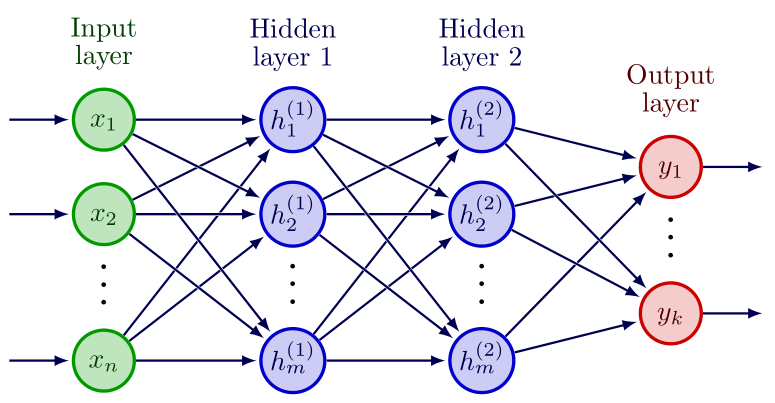
\includegraphics[width=12cm]{kapitel/2_stand_der_technik/img/neural-network.png}
	\caption[Darstellung eines Neuronalen Netzes]{Darstellung eines Neuronalen Netzes.}
	\label{img:neural-networks}
\end{figure}

Neuronale Netze bestehen aus synthetischen Neuronen, wobei sich beides am jeweiligen biologischen Vorbild orientiert.
In der Grafik \cref{img:neural-networks} sind die Neuronen als farbige Kreise gekennzeichnet.
Die Aufgabe eines Neurons besteht in der Umwandlung eines oder mehrere Eingangssignale in ein Ausgangssignal.
Für die Umwandlung wird beispielsweise die Summe aller Eingaben berechnet, auf eine Aktivierungsfunktion angewendet und an alle Ausgaben weitergegeben.
\newline

Neuronen sind in der Regel in Schichten sortiert, die jeweils mit der vorherigen Schicht verbunden sind.
Damit die Neuronen der verschiedenen Schichten miteinander kommunizieren können, gibt es Übergänge, die in \cref{img:neural-networks} als schwarze Linien dargestellt sind.
Jeder Übergang besitzt ein Gewicht, das mit dem zu übertragenden Wert multipliziert wird.
So wird die Komplexität des Modells erhöht, wodurch schwierigere Aufgaben gelöst werden können.
\newline

Die Berechnung des Ausgabewertes wird durch die folgende Formel mit dem Ausgabewert $y$, Eingaben $x$, Gewichte für die jeweiligen Eingaben $w$ und Aktivierungsfunktion $\varphi$ verdeutlicht:

\begin{equation}
	y = \varphi ( \sum_{n=0}^N x_n * w_n).
\end{equation}

\subsection{Training}
Neuronale Netze werden nicht im klassischen Sinne programmiert, stattdessen werden definierte Netzarchitekturen trainiert.
Der Trainingsprozess orientiert sich hierbei wieder an natürlichen Lernvorgängen.
Dazu gehören unter anderem Supervised- und Unsupervised-Learning.
Der Unterschied zwischen den Verfahren liegt in der Existenz eines vorgegebenen Erwartungswertes für jede Eingabe.
Beide Verfahren haben Vor- und Nachteile, ihre Anwendung ergibt sich in der Regel aus den vorliegenden Daten und gewünschten Ergebnissen.

Ziel des Trainings ist die Anpassung der Weights, der Übergänge zwischen den Neuronen.
Sie werden im Kontext des Trainingsprozesses auch Parameter genannt.
Durch die Anpassung der Parameter passt sich das Netz den Daten an und erlaubt so verschiedenste Aufgaben zu lösen.
So können dann beispielsweise Gesichter in Bildern oder Betrugsfälle in Abbuchungen erkannt werden.
\newline

Für das Training müssen zusätzliche Konfigurationen festgelegt werden, die Hyperparameter genannt werden.
Im Gegensatz zu den Parametern neuronaler Netze werden sie durch das Training nicht verändert.
Bei Hyperparametern handelt es sich zum Beispiel um die Anzahl an Neuronen in einer bestimmten Schicht \cite{hyperparameters-gan-using-genetic-algorithm}.
Die Auswahl an Hyperparametern hat einen sehr großen Einfluss auf den Trainingserfolg von Modellen.
Zusätzlich unterscheiden sich optimale Hyperparameter je nach Architektur und zugrundelegenden Daten, weswegen eine eigene Hyperparametersuche immer sinnvoll ist.
Es sind auch nicht alle Hyperparameter gleichbedeutend für den Trainingserfolg, beispielsweise die Lernrate hat einen besonders großen Einfluss auf den Trainingserfolg \cite{learning-rate-most-important}.

\subsection{Verschiedene Schichten}
Wie bereits erwähnt, werden Neuronale Netze mittels Schichten aufgebaut.
Es existieren verschiedene Typen von Schichten, welche jeweils ganz bestimmte Aufgaben übernehmen.
Die wichtigsten Arten sollen in der folgenden Aufzählung kurz erläutert werden.

\subsubsection{InputLayer und OutputLayer}
Diese beiden Schichten gehören nicht zu der Blackbox, die ein Neuronales Netz charakterisiert.
Wie man bereits in der Abbildung \ref{img:neural-networks} erkennen konnte, werden über diese beiden Schichten mit dem Modell interagiert.
Das InputLayer definiert, welche Formfaktor die zu verarbeiteten Daten haben müssen.
Diese Daten sind immer in der Form eines Tensors gegeben und können sich über mehrere Dimensionen spannen. 
So repräsentiert die Formangabe \textit{[3, 50]} eine Matrix mit drei Reihen und 50 Spalten.
Diese Formangabe spielt auch bei anderen Schichten innerhalb des Neuronalen Netzes eine Rolle.
So hat jede einzelne Schicht eine Input- und Output-Größe.
\newline

Das OutputLayer ist normalerweise keine spezielle, dedizierte Schicht.
In der Regel, repräsentiert die letzte im Modell angeschlossene Schicht die Ausgabe.

\subsubsection{DenseLayer}
Das DenseLayer ist eine so genanntes \textit{deeply connected Layer}.
Das bedeutet, dass jedes Neuron mit jedem Neuron der vorherigen Schicht verbunden ist.
Auch dies kann in der Abbildung \ref{img:neural-networks} beobachtet werden, wobei beide blauen Schichten diesem Typ entsprechen.
Diese Eigenschaft macht das DenseLayer zu einem der weitestverbreiteten Schichten innerhalb Neuronaler Netze \cite{dense-layer}.
Vor allem im Bereich der Klassifizierung wird es häufig eingesetzt.

\subsubsection{ConvolutionalLayer}
Das ConvolutionalLayer stellt eine so genannte Faltungsoperation dar.
Dabei wird eine Matrix aus Gewichten, Filter oder Kernel genannt, über den Input bewegt.
Bei jeder Position werden die Gewichte mit dem darunter liegenden Inputwert multipliziert und anschließend alle Produkte summiert \cite{convolutional_tut}.
In der Abbildung \ref{img:convelutional_layer} wird dies für eine zwei dimensionale Faltung visualisiert.

\begin{figure}[H]
	\centering
	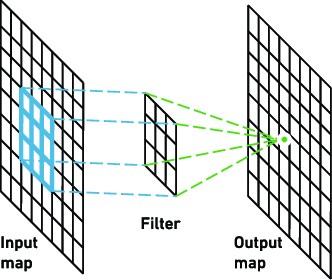
\includegraphics[width=6cm]{kapitel/2_stand_der_technik/img/convolutional_layer.png}
	\caption[Anwendung einer Faltungsoperation]{Anwendung einer Faltungsoperation \cite{convolutional-malware}}
	\label{img:convelutional_layer}
\end{figure}


Dieser Prozess kann für verschiedene Zwecke, wie der Kantendetektion in Bilder, verwendet werden.
Bei einem ConvolutionalLayer lernt das Modell die einzelnen Gewichte des Filters, um automatisch Features zu erkennen.
Den Output nennt man dann eine \textit{FeatureMap} \cite{convolutional_tut}.
\newline

In einem Convolutional Neural Network wird diese Schicht so verwendet, dass die resultierenden \textit{FeatureMap} immer kleiner werden.
Wie stark die Ausgabe minimiert wird, definieren die Kernel-Größe, Padding und Stride \cite{padding_stride}.
Durch Padding wird der Rand um die Eingabe herum aufgefüllt.
Stride gibt an, wie viele Felder die Matrix nach jeder Operation weiter springt, um so beispielsweise eine Überlappung der Faltung zu erzeugen.
Den Einfluss von verschiedenen Stride-Werten kann sehr gut in Abbildung \ref{img:convelutional_stride} erkannt werden.

\begin{figure}[H]
	\centering
	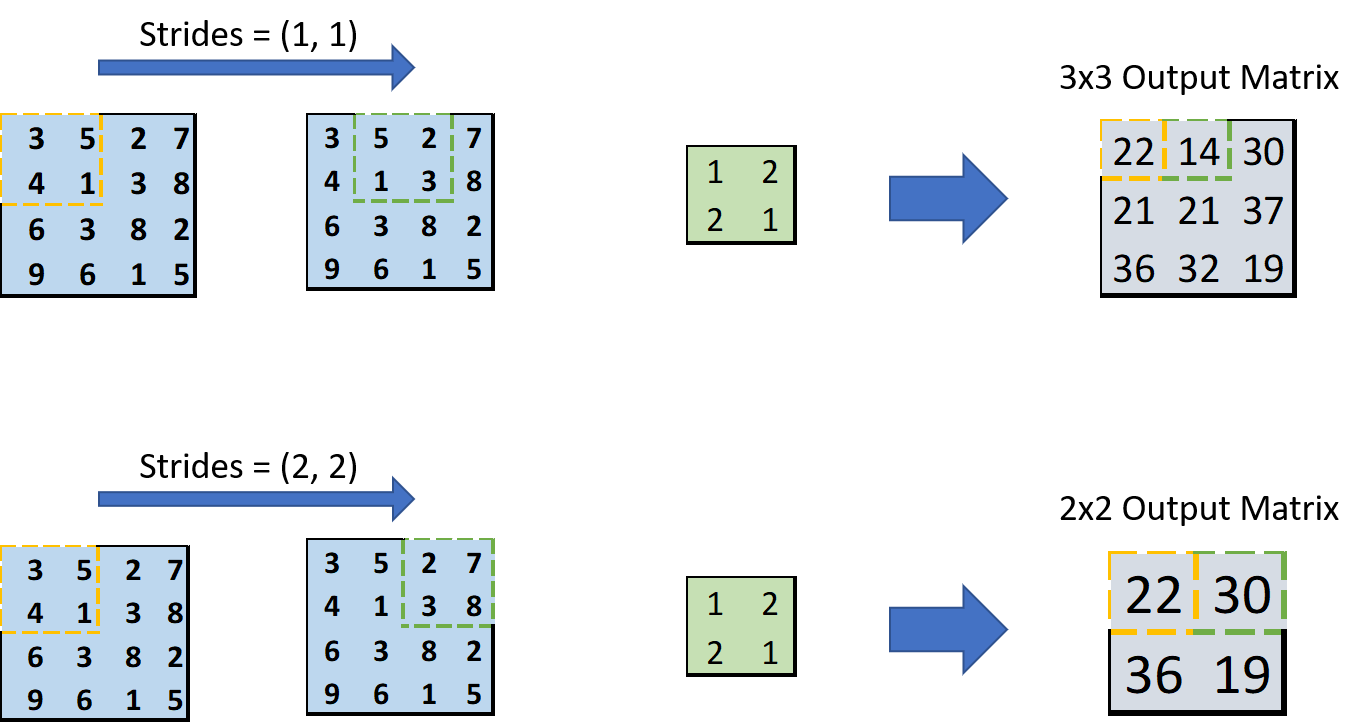
\includegraphics[width=12cm]{kapitel/2_stand_der_technik/img/stride.png}
	\caption[Ein Stride von 2 erzeugt eine kleinere Output Matrix als ein Stride von 1]{Ein Stride von 2 erzeugt eine kleinere Output Matrix als ein Stride von 1 \cite{convolutional_transpose}}
	\label{img:convelutional_stride}
\end{figure}

\subsubsection{ConvolutionalTransposeLayer}

Das Gegenstück zum ConvolutionalLayer ist das ConvolutionalTransposeLayer.
Dabei wird ein einzelner Wert aus dem Input mit jedem Gewicht des Kernels multipliziert.
Wie in der Abbildung \ref{img:convelutional_transpose_layer} zu erkennen ist, erreicht man somit einen größeren Output.

\begin{figure}[H]
	\centering
	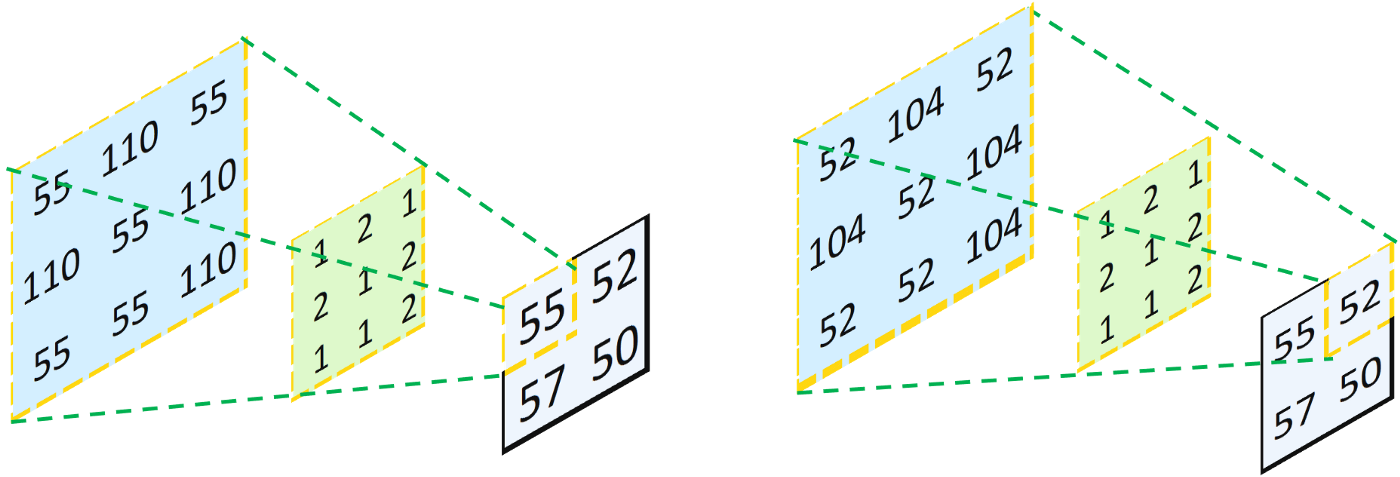
\includegraphics[width=10cm]{kapitel/2_stand_der_technik/img/convolutional_transpose_layer_cut.png}
	\caption[Die umgekehrte Faltungsoperation]{Die umgekehrte Faltungsoperation \cite{convolutional_transpose}}
	\label{img:convelutional_transpose_layer}
\end{figure}

Anschließend müssen nur noch die einzelnen Ergebnisse relativ zu ihrer ursprünglichen Position übereinander gelegt und summiert werden (siehe Abbildungs \ref{img:convelutional_transpose_layer_final}).

\begin{figure}[H]
	\centering
	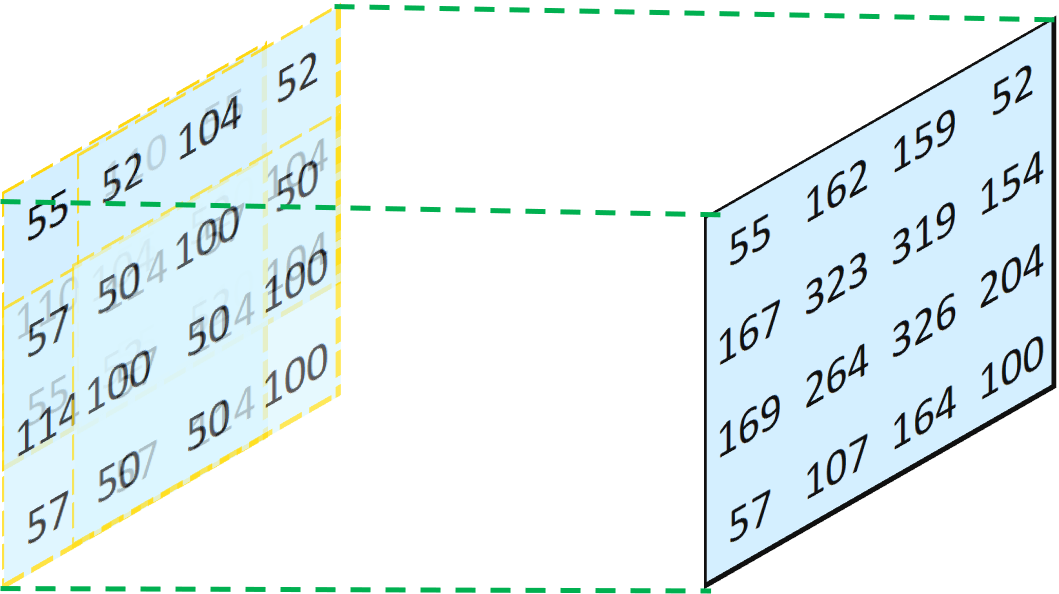
\includegraphics[width=7cm]{kapitel/2_stand_der_technik/img/convolutional_transpose_layer_final.png}
	\caption[Das Vereinigen der Ergebnisse]{Das Vereinigen der Ergebnisse \cite{convolutional_transpose}}
	\label{img:convelutional_transpose_layer_final}
\end{figure}


\subsubsection{ActivationLayer}
Aktivierungsfunktionen sind ein wichtiges Werkzeug innerhalb Neuronaler Netze.
Sie bilden ein großes Spektrum an Werten auf einen kleinen Bereich ab.
Beliebte Funktionen sind dabei LeakyReLU, Tanh oder Softmax.
Häufig kann man sie am Ende eines Modells finden.
Nicht selten stellen sie das OutputLayer eines Netzes dar.
Jedoch werden sie auch innerhalb der HiddenLayer verwendet.
Sie folgen häufig auf Dense oder ConvolutionalLayer.

\subsubsection{BatchNormalization}

Normalisierung stellt einen Schritt der Vorverarbeitung dar, bei dem die Trainingsdaten standardisiert werden.
Dabei werden die Daten gemittelt und die Standardabweichung wird auf einen immer gleichen Wert gebracht.
Bei der \textit{BatchNormalization} wird dieser Prozess innerhalb einer Schicht angewendet.
Dies lässt sich in der Abbildung \ref{img:batch-norm} erkennen.
Dabei steht das \textit{z} für den Wert, der das Neuron errechnet, \textit{a} für die Aktivierungsfunktionen der jeweiligen Schicht und die rote Linie dazwischen repräsentiert die Normalisierung.

\begin{figure}[H]
	\centering
	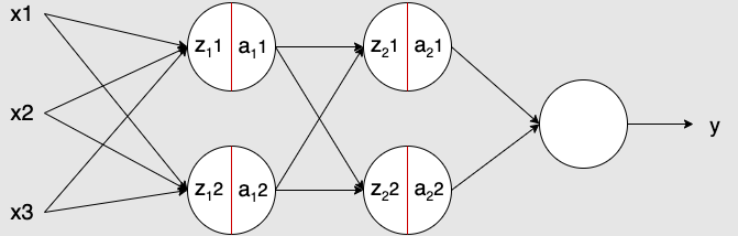
\includegraphics[width=12cm]{kapitel/2_stand_der_technik/img/batchNormalization.png}
	\caption[Anwendung der BatchNormalization]{Anwendung der BatchNormalization \cite{batch-normalization}}
	\label{img:batch-norm}
\end{figure}

\textit{BatchNormalization} soll vor allem einen Effekt namens \textit{covariate shift} unterbinden \cite{batch-normalization-paper}.
Dieser kann eintreten, sobald stark abweichende Daten vom Neuronalen Netz verarbeitet werden sollen, die das Modell noch nie gesehen hat.
Der \textit{covariate shift} beschreibt dabei, wie stark sich die Verteilung des Inputs einer Schicht plötzlich verändert.
Diese unbekannte Verteilung wird vor allem durch die erwähnten, noch nie verarbeiteten Daten ausgelöst.
Durch die Normalisierung innerhalb der Schicht, wird die Verteilung deutlich minimiert, wodurch das Training beschleunigt werden kann. 

\subsubsection{MultiplyLayer}
Diese Schicht repräsentiert, wie der Name vermuten lässt, einen arithmetischen Operator.
Es werden mehrere Input-Tensoren zu einem Output-Tensor multipliziert.
Dabei muss natürlich sichergestellt werden, das alle hineingegeben Tensoren den gleichen Formfaktor besitzen.
Diese Schicht wird eine große Rolle bei der Architekturen von GANs spielen, da dort zwei Inputs zu einem Output vereinigt werden müssen.

\section{General Adversarial Network}
Der Begriff \acrfull{GAN} ist auf Ian Goodfellow zurückzuführen \cite{gan-original-paper}.
Das Wort bezeichnet ein Konstrukt aus 2 neuronalen Netzen, die sich gegenseitig trainieren.
Durch das spezielle Training gelingt die Generierung von realistischen synthetischen Daten.
Solche Daten können dann zum Beispiel für das Training anderer neuronalen Netze \cite{gan-application-augmenting-training-data}, in der Bildverarbeitung \cite{gan-application-upscaling, gan-application-blending} und vielen weiteren Anwendungsgebieten verwendet werden \cite{gan-application-dna-optimizes-protein-functions, gan-application-audio-synthesis}.

\begin{figure}[H]
	\centering
	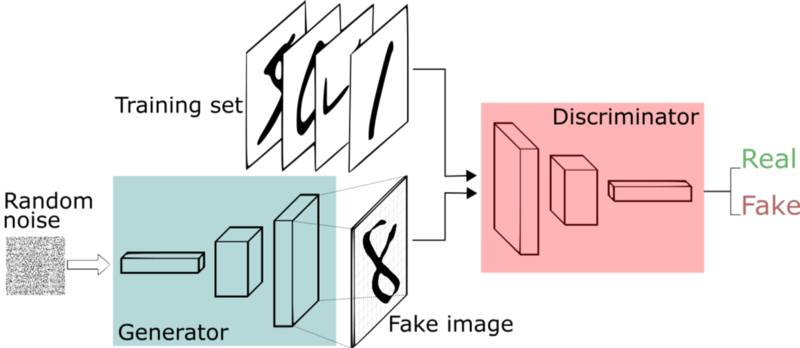
\includegraphics[width=12cm]{kapitel/2_stand_der_technik/img/GAN.png}
	\label{img:gan}
	\caption{Generative Adversarial Network (Bild von Thalles Silva \cite{img-gan})}
\end{figure}

Die beiden Netze eines \acrshort{GAN}s werden in den Generator und den Discriminator unterschieden.
Aufgabe des Generators ist die Generierung von synthetischen Daten.
Dafür wandelt er eine zufällige Eingabe in einen möglichst realistischen Output um.
Die zufällige Eingabe dient als Basis für die Ausgabedaten.
Das ist notwendig, da der Umwandlungsprozess selbst deterministisch ist, aber trotzdem eine Vielzahl an unterschiedlichen Daten generiert werden soll.
\newline

Der Output des Generators wird vom Discriminator klassifiziert.
Dafür wird er sowohl auf die generierten Daten als auch einen Bestand an echten Daten trainiert.
Sein Ziel ist es, die falschen Daten des Generators zu identifizieren.
Ziel des Generators hingegen ist es, den Discriminator zu täuschen und die generierten Daten als echt wirken zu lassen.
\newline

Ian Goodfellow bezeichnet den Lernprozess auch als Minimax-Spiel, bei dem die Ausgabe des Discriminators die zu optimierende Größe ist.
Das bedeutet, der Generator versucht die Genauigkeit des Discriminators zu verringern, während der Discriminator sie erhöhen möchte. \cite{gan-minimax}

\subsection{Ausprägungen von GANs}
In diesem Kapitel die Architekturmodelle CGAN, Dense-GAN und DC-GAN vorgestellt.
Das ist deshalb wichtig, da die zugehörigen Bezeichnungen in der Literatur nicht klar definiert sind.
So werden beispielsweise je nach Kontext der Arbeit sowohl Cycle-GANs als auch Conditional GANs als CGANs bezeichnet.

\subsubsection{CGAN}
Das \acrfull{CGAN} \cite{mirza2014conditional, gan-conditional} erlaubt die Beeinflussung der Generierung durch Labels.
Dafür wird der normale Trainingsablauf eines GANs durch Labels erweitert, wie in der Abbildung dargestellt.
\begin{figure}[H]
	\centering
	% Dokument: https://drive.google.com/file/d/1qso4iFm3YGvxG3NmwlUdatspkJdja00B/view?usp=sharing
	% beim Export auf 300% Zoom stellen
	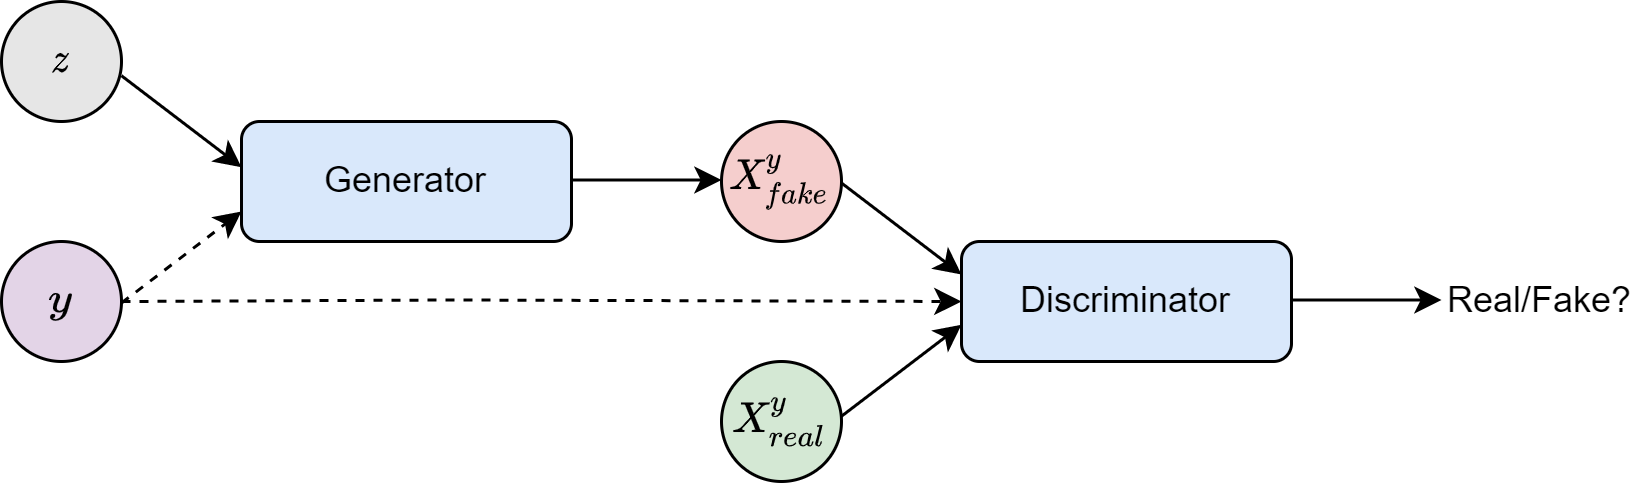
\includegraphics[width=14cm]{kapitel/2_stand_der_technik/img/cgan-vs-gan.drawio.png}
	\caption[Flowchart Trainingsprozess GAN und CGAN]{Flowchart Trainingsprozess GAN (nur durchgestrichene Pfeile) und CGAN (alle Pfeile)}
	\label{flowchart-cgan-vs-gan}
\end{figure}

Das Datenlabel $y$ wird sowohl für die Generierung der Bilder, als auch bei der Verifizierung durch den Discriminator genutzt.
Dafür erhalten sowohl Discriminator als auch Generator eine weitere Eingabe.
So kann der Discriminator den Zusammenhang zwischen Label und bestimmten Eigenschaften der Daten lernen.
Dadurch ist dann der Generator gezwungen, diese Eigenschaften zu berücksichtigen, um den Discriminator wieder zu täuschen.
\newline

Sobald das \acrshort{GAN} zufriedenstellend trainiert ist, können so labelspezifische Daten generiert werden.
Das kann in der Praxis sehr günstig sein, wenn zum Beispiel das Krankheitsbild einer bestimmten Krankheit generiert werden soll.
Die Nutzung des Conditional Discriminators erlaubt zusätzlich die Identifizierung einer bestimmten Krankheit auf einem Bild.

\subsubsection{Dense-GAN}
Eine Dense-GAN nutzt sowohl für Discriminator als auch für den Generator Dense Layer beziehungsweise Fully Connected Layer.
Dense Layer bestehen aus Neuronen, die jeweils mit jeder Ausgabe der vorherigen Schicht verknüpft sind.
\newline

Vorteil dieses Architekturmodells ist seine große Flexibilität.
Mithilfe der Dense Layer und einer ausreichend großen Architektur lassen sich theoretisch alle Zusammenhänge eines Datensets lernen.
\newline

Nachteil sind die vielen zu lernenden Parameter.
Pro Schicht ergeben sich $|weights| = inputs * outputs$, was bei größeren Architekturen einen erheblichen Lernaufwand bedeutet.
Insbesondere im Vergleich zu Convolutional Layern macht dies einen enormen Unterschied.

\subsubsection{DC-GAN}
Ein DC-GAN oder auch Deep Convolutional GAN besteht hauptsächlich aus Convolutional Layern.
Im Generator finden vor allem Convolutional Transposed Layer ihre Anwendung.
Convolutional Transpose Layer funktionieren wie Convolutional Layer, jedoch vergrößern sie Ausschnitte, statt sie zu komprimieren.
Im Discriminator werden Convolutional Layer genutzt, um die Datenmenge auf eine Entscheidung klein zu skalieren.
Im letzten Schritt des Discriminators existiert in der Regel ein Dense Layer, um die finale Entscheidung zu berechnen.
\newline

Vorteil dieser Architektur sind die vergleichsweise wenigen zu lernenden Parameter.
Die geringe Anzahl an Parametern sind der Tatsache geschuldet, dass es pro Ausgabe-Dimension nur einen Filter für das Convolutional Layers gibt.
Dadurch ist auch die Parameteranzahl der Convolutional Layer unabhängig von der Bildgröße.

Zusätzlich zur geringen Parameteranzahl fördern die Filter auch das Verständnis von Zusammenhängen zwischen benachbarten Pixeln.
Die Zusammenhänge werden dabei implizit durch die Architektur vorgegeben und müssen nicht erst aufwändig gelernt werden.
\newline

Die Tatsache, dass die Filter der Convolutional Layer Zusammenhänge zwischen benachbarten Datenpunkten implizieren ist auch gleichzeitig ein Nachteil der Architektur.
Sollten die Beziehungen zwischen nahen Datenpunkten nicht existieren, können falsche Zusammenhänge vorausgesetzt werden, was zu schlechteren Ergebnissen führen kann.
Insgesamt ist eine solche Architektur somit nicht so flexibel wie eine Dense Architektur, aber dafür effizienter.

\section{Metriken}
\subsection{FID}	
% TODO quelle: https://wandb.ai/ayush-thakur/gan-evaluation/reports/How-to-Evaluate-GANs-using-Frechet-Inception-Distance-FID---Vmlldzo0MTAxOTI
Die Bewertung von Trainingserfolgen durch GANs ist nicht trivial, denn für die Bewertung muss die Qualität der generierten Bilder eingeschätzt werden.
Erstmals in \cite{fid} wurde dafür der \acrfull{FID} aufgezeigt.

Für die Berechnung des \acrshort{FID} werden zunächst die Ausgaben eines Layers des Inception Nets von Trainingsdaten und generierte Daten gesammelt.
Danach wird aus den Werten der Embeddingschicht der Durchschnitt und die Kovarianz berechnet und verrechnet.
Die nachfolgende Formel \cite{are-gans-created-equally} zeigt die genaue Berechnung auf, wobei sich $x$ und $g$ auf die Trainingsdaten und genierten Daten beziehen

\begin{equation}
	\FID(x, g) = ||\mu_x - \mu_g||_2^2 + \Tr(\Sigma_x + \Sigma_g - 2(\Sigma_x \Sigma_g)^{\frac{1}{2}}).
\end{equation}

Die \acrshort{FID} erlaubt die Einschätzung der Qualität der Bilder korrelierend zu menschlichen Einschätzungen.
% TODO mode collapse erklären
Auch die Vielfalt wird bewertet, indem zum Beispiel Mode-Collaps als negativ bewertet wird und gleichzeitig eine relative Robustheit gegenüber Rauschen besteht (im Vergleich zum Inception Score \cite{are-gans-created-equally}). 

\begin{figure}[H]
	\centering
	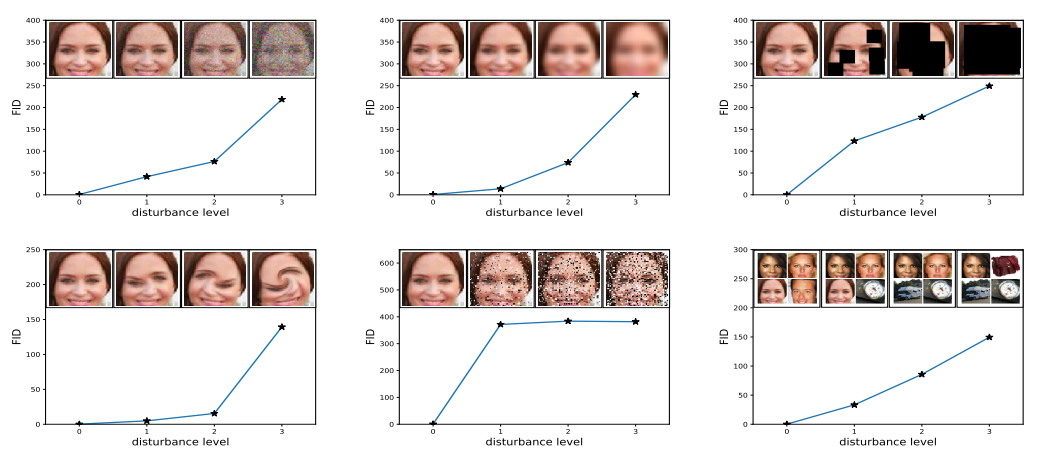
\includegraphics[width=16cm]{kapitel/2_stand_der_technik/img/fid-example.png}
	\caption[Beispiel von unterschiedlichen FID-Werten]{Beispiele unterschiedlicher FID-Werte aus \cite{fid}.\\ \textbf{Oben Links:} gaußsches Rauschen; \textbf{Oben Mitte:} gaußscher Weichzeichner; \textbf{Oben Rechts:} schwarze Rechtecke; \textbf{Unten Links:} verwirbelte Bilder; \textbf{Unten Mitte:} Salt and Pepper Noise; \textbf{Unten Rechts:} CelebA Datensatz mit ImageNet Bildern versetzt }
	\label{fid-example}
\end{figure}

\section{Hyperparameter}
\todo{was ist ein hyperparemter?}
\subsection{Auswahl an Hyperparametern}

\subsubsection{Learning-Rate}
Die Learning-Rate entspricht dem Faktor \(\alpha\), welcher die Intensität des Gradientenabstiegs bestimmt:  
\begin{equation}
	\theta  =  \theta  - \alpha   \nabla_{ \theta }  J( \theta ).
\end{equation}

\todo[]{mit quellen backen}
Bei zu großem \(\alpha\) kann der Trainings-Fehler anfangen zu oszillieren oder sogar größer werden.
Bei zu kleinem \(\alpha\) konvergiert der Fehler zu langsam oder bleibt in einem lokalen Minimum stehen. 
Es ist anzumerken, dass die oben gezeigt Formel dem einfachen Gradientenabstieg entspricht.
Normalerweise werden fortgeschrittenere Algorithmen angewendet, welche jedoch weiterhin auf dem Gradientenabstieg basieren.
So können weitere Parameter, wie das \textit{Momentum} die Abstiegsweite beeinflussen.
\newline

Für alle Architekturen wird der Adam-Optimierungs-Algorithmus angewendet.
\todo{warum? 1. bekannt / standart, 2. schnelle ergebnisse}
\todo{wie funktioniert er grob?}

\subsubsection{Batch-Size}
Ähnlich wie die Learning-Rate ist auch die Batch-Size ein sehr beliebter Hyperparameter und wird in unterschiedlichen Tutorials referenziert \cite{tutorial:tune-batch-size-analyticsvidhya, tutorial:tune-batch-size-machinelearningmastery}.
Die Batch-Size beschreibt, wie viele Traingsdaten verabeitet werden, um einen Gradientenabstieg der Gewichte durchzuführen.
Grundsätzlich führt eine kleine Batch-Size zu besseren Ergebnissen.
Ein Experiment über kleine Batch-Größen im Bezug auf Neuronale Netze kam zu folgenden Ergebnis: 

\begin{displayquote}
	\enquote{In all cases the best results have been obtained with batch sizes m = 32 or smaller, often as small as m = 2 or m = 4.}
	\cite[S. 16, Z. 5-7]{small-batch-size}
\end{displayquote}

Eine kleinere Batch-Size führt dazu, dass der Fehler speziellere Fälle abbilden kann und damit eine Generalisierung unterbunden wird \cite{tutorial:tune-batch-size-machinelearningmastery}.
Jedoch ergibt sich aus einer kleineren Batch-Size ein Leistungs-Problem: die Berechnung des Fehlerwerts und die anschließende Optimierung der Gewichte wird häufiger durchgeführt.
Das führt logischerweise zu einer längeren Trainingsdauer pro Epoche.

\subsubsection{Dropout}
Der Dropout definiert die Größe eines zufälligen Anteils an Neuronen, die dann inklusive ihrer Verbindungen im Training deaktiviert werden.
Das führt dazu, dass immer andere Neuronen das Ergebnis beeinflussen, was Overfitting entgegenwirkt \cite{JMLR:v15:srivastava14a}.
Bei Overfitting lernt das neuronale Netz Besonderheiten der Trainingsdaten, die aber in der Realität nicht vorkommen.
Dadurch erzielt es sehr gute Ergebnisse im Training, spätestens bei der Anwendung ist die Leistung jedoch verhältnismäßig schlecht.

% TODO https://machinelearningmastery.com/dropout-for-regularizing-deep-neural-networks/

\subsubsection{Smoothness - Onesided Label Smoothing}
Onesided Label Smoothing entstammt einer Idee von Ian Goodfellow \cite{ian-goodfellow-onesided-label-smoothing}.
Sie verändert den Loss, indem sie den Optimalwert für das gewünschte Ergebnis anpasst.
Dafür wird die optimale Ausgabe des Discriminators von 1 oder 0 auf beispielsweise 0.9 oder 0.1 gesetzt.
Der Prozess hilft besonders gegen Adversarial Examples.
Adversarial Examples sind sehr geringe Unterschiede in den Bildern, die die Klassifikation des Discriminators aber sehr stark beeinflussen.
Sollte der Generator diese Änderungen lernen, kann er den Discriminator täuschen, ohne dass sich die Bildqualität erhöht.

\begin{figure}[H]
	\centering
	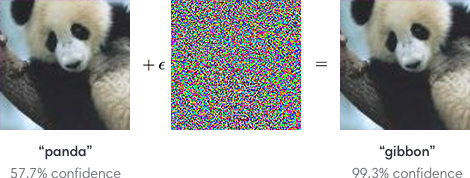
\includegraphics[width=10cm]{kapitel/2_stand_der_technik/img/adversrial-example.png}
	\caption[Adversarial Example]{Durch das (für Menschen nicht erkennbare) zusammenführen der 2 Bilder, wird der Panda fälschlicherweise als Gibbon klassifiziert \cite{example-one-sided-label-smoothing}}
	\label{smoothness-adversarial-example}
\end{figure}

\todo{Smoothness durch Onesided Label Smoothing ersetzen oder erklären, dass beides das gleiche ist?}

\subsection{Verfahren zur Bestimmung von Hyperparametern}
\label{chapter:verfahren-bestimmung-hyperparameter}
\todo{Quelle \cite{hyperparameters-search}}

Die Bestimmung guter Hyperparameter ist im Rahmen der Arbeit von großer Bedeutung, da verschiedene Architekturen auf ihre Effektivität und Effizienz untersucht werden sollen.
Der Vergleich verschiedener Architekturen mit gleichen Hyperparametern ist hingegen nicht fair, da der Einfluss der Hyperparameter auf das Ergebnis so groß ist.
\newline

Für die Suche nach optimalen Hyperparametern gibt es verschieden Verfahren, die im Folgend vorgestellt werden.
Dabei wird sich auf die Grid Search, Random Search und den Genetic Algorithm beschränkt, da diese die beliebtesten Algorithmen zur Optimierung sind \cite{hyperparameters-search-comparison-focus-genetic}.
Die Verfahren werden zusätzlich mit der manuellen Suche verglichen, um eine allgemeinere Einschätzung gewährleisten zu können.

\subsubsection{Manuelle Suche}
Die manuelle Suche ist das simpelste vorgestellt Verfahren.
Hierfür werden nur die Hyperparameter vor jedem Training manuell festgelegt.
Nach einem Trainingsdurchlauf können dann die Ergebnisse analysiert, Hyperparameter angepasst und die verbesserte Version erneut trainiert werden.

%Die manuelle Suche ist vor allem bei unwichtigen Hyperparametern sinnvoll, da dort bekannte Standardwerte gesetzt werden können.
%Für eine gründliche Suche aller Hyperparameter ist die manuelle Suche allerdings viel zu aufwändig.

\subsubsection{Grid Search}
Bei der Grid Search \cite{hyperparameters-grid-search} werden zunächst die zu untersuchenden Hyperparameter ausgewählt.
Danach erfolgt die Definition eines Suchintervalls inklusive Intervallschritten für jeden Hyperparameter.
Schließlich wird das neuronale Netzwerk für jede Kombination der Hyperparameterwerte trainiert und die Ergebnisse der einzelnen Durchläufe festgehalten.
Die Trainingsdurchläufe können dabei parallel stattfinden.

Nach dem Training ist es dann möglich, die einzelnen Ergebnisse zu vergleichen.
Dabei können dann Schemata erkannt und Kombinationen aussortiert werden.
%Es ist dann möglich die erfolgversprechendsten Netze weiter zu trainieren, oder direkt eine zufriedenstellende Kombination auszuwählen.
\newline

Insgesamt ist Grid Search sehr simpel zu implementieren, aber auch sehr ressourcenaufwändig.
Der exakte Aufwand hängt dabei stark von der Anzahl der möglichen Kombinationen der Hyperparameterwerte ab.
Da die Anzahl der Kombinationen der Hyperparameter exponentiell \todo{begründen?} wächst, nimmt auch der Aufwand mit der Anzahl an Werten sehr stark zu.
Durch die Möglichkeit von Parallelisierung findet die Grid Search in der Regel bessere Parameter als die sequentielle manuelle Suche in der gleichen Zeit \cite{hyperparameters-random-search}.

\subsubsection{Random Search}
Die Random Search \cite{hyperparameters-random-search} funktioniert ähnlich wie die Grid Search, nur werden zufällige Werte statt einem festgelegten Werteraster erzeugt.
Die zufälligen Werte haben den Vorteil, dass es weniger Werte-Überlagerungen im Vergleich zur den Raster-Kombinationen gibt, wie in \cref{randomsearch-vs-gridsearch} dargestellt.
Deswegen kann die zufällige Suche bei gleich vielen Durchläufen ein größeres Spektrum an Ergebnissen abdecken.
Mittels \textit{Automatic Relevance Determination} \cite{automatic-relevance-determination} ist es dann möglich, den Einfluss und Wertebereich der einzelnen Hyperparameter darzustellen.

\begin{figure}[H]
	\centering
	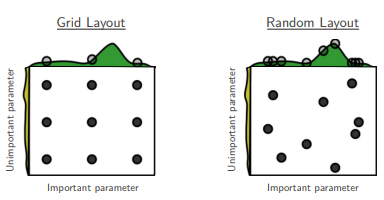
\includegraphics[width=10cm]{kapitel/2_stand_der_technik/img/random-vs-grid-search1.png}
	\caption[Vergleich zwischen Grid Search und Random Search]{
		Abbildung von 9 Optimierungsversuche der Funktion $f(x,y)=g(x)+h(x) \approx g(x)$.
		Über den Quadraten ist $g(x)$ und links $h(x)$ abgebildet.
		Während die Grid Search im Versuch nur 3 unterschiedliche Werte austestet, schafft die Random Search eine Suche über 9 verschiedene Punkte.
		\cite{hyperparameters-random-search}}
	\label{randomsearch-vs-gridsearch}
\end{figure}

Vorteil der Random Search im Vergleich zur Grid Search ist, dass keine Hyperparameter festgelegt werden müssen.
Das erlaubt eine unvoreingenommene Herangehensweise an die Suche.
\newline

Problem der Random Search ist vor allem, dass die Räume der guten Hyperparameter (\textit{Search Space}) sehr klein sind.
Dadurch ist nicht gewährleistet, dass ein zufälliger Wert auch den Raum der optimalen Werte trifft.
Jedoch erzielen Hyperparametersuchen mittels Random Search in der Regel trotzdem gute Ergebnisse.
Dem Grid Search Verfahren ist die Random Search allerdings nicht prinzipiell überlegen \cite{hyperparameters-random-search}.
\newline

Aufgrund ihrer Ähnlichkeit teilt sich die Random Search auch das Problem der Ressourcenintensivität mit der Grid Search.
Sobald ein sehr großes Spektrum an Hyperparametern untersucht werden soll, benötigt sie sehr viel Zeit.
Je nach zusätzlichen Optimierungen für die Wahl der Zufallswerte lässt sich die Random Search auch nicht unbedingt parallelisieren, was zu einer sehr langen Laufzeit führen kann.

\subsubsection{Genetic Algorithm}
Der Genetic Algorithm \cite{hyperparameters-genetic-algorithm} wandelt die Hyperparametersuche in einen evolutionären Entwicklungsprozess um.
Der Evolutionsaspekt des Algorithmus ist dabei eine Anlehnung an die natürliche Entwicklung in der Natur.
Diese Entwicklung zeichnet sich durch die Operatoren \textit{Selektion}, \textit{Kombination} und \textit{Mutation} aus, die der Algorithmus verwendet .
\newline

Für den Optimierungsprozess werden am Anfang mehrere zufällige Hyperparameterinstanzen erzeugt.
Die Instanzen werden dann trainiert und stehen im Wettbewerb um das beste Ergebnis.
Nach der Auswertung der Trainingsergebnisse werden die besten Instanzen selektiert und miteinander gekreuzt und oder mutiert.
\newline

Der Genetic Algorithm eignet sich besonders gut bei sehr vielen Hyperparametern.
Im Gegensatz zur Grid Search werden nicht immer alle Kombinationen ausprobiert, sondern nur einzelne, die sich bereits zuvor als vielversprechend herausgestellt haben.
Dadurch kann mit sehr großen Mengen an Hyperparametern umgegangen werden.
\newline

Allerdings ist der Genetic Algorithm vergleichsweise langsam, da die Evolutionsschritte sequentiell ablaufen müssen.
Erst bei einer hohen Anzahl an Hyperparametern oder einem sehr großen Suchraum ist der Genetic Algorithm effizienter als eine Grid Search \cite{hyperparameters-search-comparison-focus-genetic}.

\section{DeepLearning Framework}
Die Implementierung von DeepLearning-Algorithmen ist im Bereich der Künstlichen Intelligenzen eine bedeutende Thematik.
Vor allem die effiziente Ausnutzungen gegebener Hardware stellt eine enorme Herausforderung dar. 
Deshalb existieren über verschiedene Abstraktions-Level diverse Frameworks und Bibliotheken, welche die Arbeit deutlich erleichtern.
\newline

Aufgrund der hohen Rechenkern-Anzahl und der daraus resultierende Multithreading-Charakteristik, eignen sich Grafikkarten besonders gut für DeepLearning-Berechnungen \cite{gpu-for-dl}.
Grafikarten Hersteller stellen dafür Low-Level-APIs bereit, in denen Routinen wie Matrix-Multiplikationen oder Aktivierungs-Funktionen hardware-beschleunigt werden.
Dabei kann in den Zugang zu allgemeinen GPU-Operationen (API-Beispiel: CUDA) oder speziellen Funktionen für DeepLearning und Neuronale Netze (API-Beispiel: cuDNN) unterschieden werden.
\newline

Als Entwickler von DeepLearning-Anwendungen sind jedoch solche hardwarenahen Aufrufe häufig zu aufwendig.
Deshalb haben sich in der Industrie und Forschung DeepLearning Frameworks entwickelt, welche Algorithmen weiter zusammenfassen und abstrahieren.
Zu den am weitesten verbreiteten gehören unter anderem PyTorch, Caffe, TensorFlow und MXNet \cite{dl-framework-evaluation}. \todo{bessere quelle}
Auch wenn sie sich einige architektonische Ansätze teilen, unterscheiden sich die Frameworks jedoch in der genauen Implementierung und Technik \cite{dl-framework-evaluation}.
Der größte Unterschied ist jedoch die Popularität der Frameworks.
Gemessen an Github Sternen sind TensorFlow (164k) \cite{github-tensorflow} und PyTorch (55k) \cite{github-pytorch} die bekanntesten, weshalb sie im Folgenden näher analysiert werden.

\subsection{TensorFlow und PyTorch}
%TODO in Methodik?
TensorFlow und PyTorch weichen in einigen technischen Eigenschaften, wie der Graphen Definition und dem verteilten Training von aneinander ab \cite{pytorch-vs-tensorflow}.
Allerdings sind diese Charakteristiken im Rahmen der allgemeinen Architektur Untersuchung wenig relevant.
Für die Evaluierung selbst ist eine gute Visualisierung der Trainingsdaten und -ergebnisse wichtig.
Außerdem soll die Schnittstelle möglichst einfach sein, damit ohne großen Aufwand verschiedene Architekturen implementiert und getestet werden können.
Mittels Tensorboard bietet Tensorflow hierbei eine natives und sehr umfangreiches Werkzeug an.
PyTorch besitzt keine vergleichbaren Funktionen, stattdessen gibt es einen offiziellen Anleitungsartikel zur Integration mit Tensorboard \cite{pytorch-tensorboard-offical-documentation}.

Aufgrund der nativen Unterstützung von Tensorboard wurde sich für TensorFlow als DeepLearning Framework entschieden.

\subsection{Tensorboard}
Hinsichtlich der Visualisierung bietet TensorFlow das direkt integrierte Tensorboard.
Ohne großen Mehraufwand können so Metriken visualisiert, Modell-Graphen dargestellt oder generierte Bilder verglichen werden \cite{tensorboard}.
PyTorch besitzt keine vergleichbaren nativen Visualisierungstool, aber eine Möglichkeit zur Darstellung in Tensorboard.

\subsection{Keras}
Zwar ist TensorFlow im Vergleich zu CUDA bereits eine High-Level-API, allerdings fallen die API-Aufrufe weiterhin sehr detailliert aus.
Dadurch sind hoch flexible Modelle und Training-Loops möglich.
Bei optimierten Anwendungen garantiert das große Freiheiten, ist jedoch im Rahmen der Studienarbeit zu umständlich und komplex.
Da in dieser Arbeit grundlegende Architekturen untersucht werden sollen, wird zusätzlich die Keras API \cite{keras} verwendet.
Ursprünglich als unabhängiges Framework entwickelt, ist Keras seit TensorFlow 2.0 ein fester Bestandteil der Bibliothek.
Keras stellt eine weitere Abstraktion-Stufe dar, wodurch Modelle sehr einfach beschrieben und vordefinierte Traings-Loops verwendet werden können.

\section{Related Work}
\label{chapter:related-work}
Da die verwendeten Daten selbstständig generiert sind, gibt es keine anderen Arbeiten, die sich mit exakt den gleichen Daten beschäftigen.
In diesem Kapitel werden stattdessen Arbeiten vorgestellt, die sich mit ähnlichen Daten beschäftigen.
Ähnlichkeit ist insbesondere bei der Bildgröße und Anzahl der Farbekanäle wichtig, da ansonsten die Architekturen zu stark angepasst werden müssen, um sie auf den generierten Datensatz anzuwenden.

\subsection{CGAN - MNIST}
Das Paper \textit{Conditional Generative Adversarial Nets} \cite{mirza2014conditional} befasst sich allgemein mit der Erweiterung von GANs durch Bedingungen.
Die vorgestellten CGANs werden hierfür auf die Datensets MNIST und Flickr trainiert.
Ziel ist dabei nicht, eine optimale Netzarchitektur oder Ergebnisse zu erzielen.
Stattdessen stellt die Arbeit einen Machbarkeitsbeweis für CGANs im Allgemeinen dar.
\newline

Auf dem Paper aufbauend existiert ein Tutorial Notebook \cite{inspiration-dense-and-dc-gan}, noch einmal explizit für das MNIST Datenset.
Das ist zwar der gleiche Datensatz, der auch im Paper genutzt wird, jedoch wird dort die genaue Netzarchitektur nur grob beschrieben.
Das Notebook hingegen enthält sogar Codebeispiele in Tensorflow, die eine Beispielimplementation bilden.
\newline

Die Architekturen von sowohl dem Generator, als auch vom Discriminator bestehen ausschließlich aus Dense Layern.
Auf jede Dense Layer Schicht wird dann zusätzlich LeakyReLU und BatchNormalization angewendet.
Als Eingabe erhält der Generator zum einen die Latent Dimension mit 100 zufälligen Zahlen und als Condition eine one-hot Vektor mit 10 Zahlen, die den MNIST-Zahlen-Klassen entsprechen.
Nach 100 Epochen Training erreicht diese Architektur die folgenden Ergebnisse \todo{bei genug Seiten (inklusive Bild) raus nehmen, weil eigentlich ist das irrelevant}:

\begin{figure}[H]
	\centering
	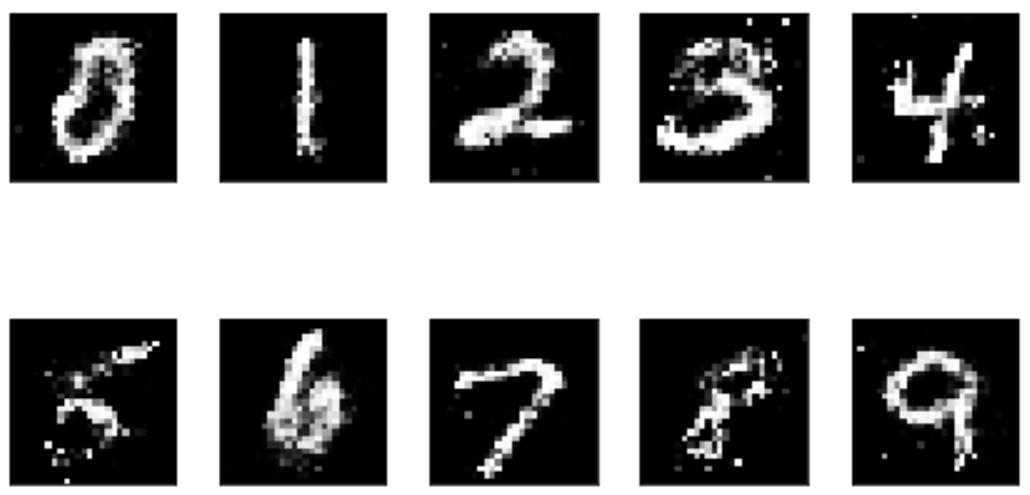
\includegraphics[width=7cm]{kapitel/2_stand_der_technik/img/cgan-notebook-ergebnisse.png}
	\caption{Ergebnisse Notebook \cite{inspiration-dense-and-dc-gan}) }
\end{figure}



\begin{comment}
	
\paragraph{Links}
\begin{itemize}
	\item Inception Score zum Rating von erzeugten Bildern (Salimans et al. 2016)
	\item Frechet Inception Distance (Heusel et al. 2017)
	\item stackoverflow \url{https://stackoverflow.com/questions/46386948/adjusting-gan-hyperparameters}
	\item \url{https://openreview.net/pdf?id=rkGG6s0qKQ}
	\item \url{https://arxiv.org/pdf/1511.06434.pdf%C3%AF%C2%BC%E2%80%B0}
	\item Forget the Learning Rate, Decay Loss \url{https://arxiv.org/ftp/arxiv/papers/1905/1905.00094.pdf}
	\item beste learningRate/Dropout/BatchSize/NumberOfNeuronsInDenseLayer mit evolutionären neuronalen netz für mnist 
	\item zum orientieren ?? \cite{gan-conditional}
\end{itemize}


\end{comment}
	% !TEX root = ../../main.tex
% !TeX spellcheck = de_DE

\chapter{Methodik}
In diesem Kapitel werden zunächst Eigenschaften der Trainingsdaten erläutert.
Dabei wird auf die Bildeigenschaften und Besonderheiten der dargestellten Figuren in den Bildern eingegangen.
Danach erfolgt eine Festlegung der Kriterien für ein erfolgreiche trainiertes 'GAN', das Grundlage für spätere Vergleiche von Trainingserfolgen sein wird.

\section{Trainingsdaten}
\todo[inline, shadow]{Rechenkapazität mit einbringen $\rightarrow$ Kompromiss von der Größe oder durch MNIST begründen?}
Das Dataset wurde im Rahmen der Studienarbeit generiert und besteht für das Training aus 1500 Bildern.
Die 1500 Bilder teilen sich dabei in jeweils 500 Bilder pro Formklasse (Dreieck, Kreis, Quadrat) auf.

\subsection{Generierung}
Bei den Trainingsdaten handelt es sich um synthetisch generierte Bilder mit geometrischen Figuren. 
Zwar gibt es bereits Datensätze mit ähnlichen Bildern \cite{dataset:2d-geometric-shapes-dataset, dataset:four-shapes}, im Rahmen der Studienarbeit werden jedoch keine vorgefertigten Datensätze verwendet. 
Denn die Generierung eigener Bilder erlaubt eine größere Kontrolle über Eigenschaften der Bilder und Inhalte, als vorgefertigte Sets.
Damit trotzdem eine Vergleichbarkeit zu anderen Arbeiten gewährleistet werden kann, wird die Generierung deterministisch reproduzierbar und dokumentiert sein.

\subsection{Eigenschaften}
Alle Bilder haben eine Größe von 28x28 Pixel und sind Schwarz-Weiß kodiert.
Der Grauwert jedes Pixels wird durch einen Channel angegeben, dessen Werte durch eine Zahl im ganzzahligen Intervall $[0; 255]$ festgelegt ist.
Dabei entspricht die Zahl 0 einem schwarzen Pixel und die Zahl 255 repräsentiert einen weißen Pixel.
\newline

Auf jedem Bild ist eine geometrische Form abgebildet.
Bei den geometrischen Formen handelt es sich um gleichseitige Dreiecke, Quadrate und Kreise.
Die Formen unterscheiden sich in Größe und Position auf dem Bild.
Andere Transformationen, wie beispielsweise Rotationen, werden nicht angewendet.
\newline

Die Quadrate und gleichseitigen Dreiecke sind zwischen 5 und 16 Pixel groß.
Die Größe bezieht sich dabei auf die Seitenlänge der Seiten.
Die Kreise sind zwischen 5 und 10 Pixel groß.
Hierbei gibt der Wert den Radius des Kreises an.
\newline

Die Formen sind so im Bild positioniert, dass sie Seitenränder touchieren können.
Allerdings ist eine Form immer vollständig im Bild abgebildet und wird vom Bildrand nicht geschnitten.

\newcommand{\trainDataImage}[1]{\subfloat{\fbox{\includegraphics{#1}}}}
\begin{figure}[H]
	\centering
	\trainDataImage{kapitel/3\_methodik/data/circle\_00.png}
	\trainDataImage{kapitel/3\_methodik/data/circle\_01.png}
	\trainDataImage{kapitel/3\_methodik/data/circle\_02.png}\par 
	
	\trainDataImage{kapitel/3\_methodik/data/rectangle\_00.png}
	\trainDataImage{kapitel/3\_methodik/data/rectangle\_01.png}
	\trainDataImage{kapitel/3\_methodik/data/rectangle\_02.png}\par 
	
	\trainDataImage{kapitel/3\_methodik/data/triangle\_00.png}
	\trainDataImage{kapitel/3\_methodik/data/triangle\_01.png}
	\trainDataImage{kapitel/3\_methodik/data/triangle\_02.png}\par 
	
	\caption{Auswahl an zufällig generierten Trainingsbilder}
\end{figure}

\section{Architekturen}
\subsection{API}
Um alle möglichen Architekturen in das Training einbinden zu können müssen sie die gleichen Ein- und Ausgaben besitzen.
Die Anforderungen an die Ein- und Ausgabe wie folgt definiert.
\newline

Der Generator erhält als Eingabe einen 100 Stellen langes Array mit Zufallszahlen (Latent-Dimension) und eine Zahl zwischen 0 und 2, die das Label repräsentiert.
Die Ausgabe des Generators ist ein Array mit den gleichen Dimensionen, wie ein Bild (28x28x1).
\newline

Der Discriminator erhält als Eingabe ein Bild als Array und zusätzlich ein Label als Zahl.
Die Ausgabe ist eine Zahl zwischen 1 und -1, die die vorhergesagte Echtheit angibt.

\section{Verfahren zur Hyperparametersuche}
\todo[shadow,inline]{Aufbau ändern in: Kriterien $\rightarrow$ Tabelle $\rightarrow$ Auswahl/Bewertung (siehe Kommentare)}
Zur Auswahl von Hyperparametern gibt es verschiedene Verfahren.
Dazu gehören unter anderem die Manuelle Suche, Grid Search, Random Search und Genetic Algorithms (siehe \cref{chapter:verfahren-bestimmung-hyperparameter}).
In diesem Abschnitt werden die verschiedenen Verfahren verglichen und zusätzliche Anpassungen erläutert.

\subsection{Kriterien}
\todo[inline, shadow]{irgendwo hardware festhalten}
In diesem Abschnitt werden Kriterien für die Auswahl eines geeigneten Hyperparameter Suchverfahrens ausgewählt.
Die Kriterien dienen als Basis für die Bewertung der Suchverfahren im nächsten Schritt.

\paragraphNewLine{Automatisierbarkeit}
Ziel ist es, pro Nacht eine Architektur zu trainieren.
Deswegen ist es wichtig, dass das Verfahren vollkommen automatisiert ablaufen kann.

\paragraphNewLine{Ressourcenbedarf}
Das Verfahren darf in keinem Fall während oder nach einer Trainingsiteration so viel zusätzlichen Speicher belegen, dass das Training fehlschlägt.
Denn Trainingsabläufe sollen primär über Nacht durchgeführt werden, wodurch Fehlschläge erst sehr spät entdeckt werden.

Dabei ist zu beachten, dass die Hardware den Trainingsprozess stark beeinflusst.
So ist der verfügbare Arbeits- und Grafikkartenspeicher nicht ausreichend, um Trainingsdurchläufe stark zu parallelisieren.

\paragraphNewLine{Laufzeit}
Die Laufzeit der Hyperparametersuche ist von entscheidender Bedeutung.
Denn die verwendete Hardware ist nicht ausreichend, um jegliche Kombinationen von Hyperparametern in einer vernünftigen Zeit zu testen.
Als zeitliche Begrenzung dient dabei die Ausführung in einer Nacht von 8h.

Jedoch ist zu beachten, dass auch der Trainingsprozess als solcher viel Zeit in Anspruch nimmt.
Der reine Trainingsaufwand erlaubt mit der verwendeten Hardware in den 8h maximal 75 sequentielle Trainingsdurchläufe (je nach Architektur kann der genaue Wert abweichen).
Folglich sollte das Verfahren innerhalb von 75 Durchläufen zu einem Ergebnis kommen.

\paragraphNewLine{Effektivität}
Das Verfahren soll in jedem Fall eine gute Kombination im zeitlichen Rahmen finden.
Das ist insofern wichtig, als dass ansonsten kein Vergleich zu anderen Architekturen erfolgen kann.
Aufgrund der geringen Ressourcen (Zeit und Rechenleistung) besteht zwar kein Anspruch auf Optimalität, jedoch sollte es zumindest ein gutes Ergebnis liefern.

\paragraphNewLine{Implementierungsaufwand}
Der zusätzlich verursachte Implementierungsaufwand ist nicht so wichtig wie die anderen Kriterien.
Er kann aber als Ausschlusskriterium bei ähnlich guten Verfahren dienen.
Der Implementierungsaufwand wird durch Dokumentation, Tutorials, Libraries, oder eine Einbindung in Tensorflow/-board verringert.

Bei der Verwendung von Libraries ist essentiell, dass sie eigene Trainingsfunktionen und den spezielleren Trainingsablauf von GANs unterstützen.
Zusätzlich müssen sie in jedem Fall mit Tensorflow oder Keras kompatibel sein.

\subsection{Vergleich}
In diesem Abschnitt werden die vorgestellten Verfahren miteinander auf Basis der Kriterien verglichen.

\paragraphNewLine{Manuelle Suche}
Die manuelle Suche ist aufgrund der ständigen verpflichtenden Neuevaluierungen der Traingsergebnisse als einziges Verfahren \todo{reicht es nur automatisierbarkeit nur in der manuellen suche anzusprechen?} nicht automatisierbar.
Zudem erhöhen die Evaluierungen den Zeitaufwand zusätzlich, da jedes mal eine fundierte\todo{mehr richtung durchdachte?} Entscheidung getroffen werden muss.
Insgesamt erhöht sich so die Laufzeit im Vergleich zu automatisierten Verfahren sehr stark.
\newline

Alle anderen Kriterien werden hingegen optimal erfüllt.
Denn für die Einführung einer manuellen Suche müssen keinerlei Anpassungen am Trainingsprozess oder Code vorgenommen werden.

\paragraphNewLine{Grid Search}
Die Laufzeit der Grid Search hängt stark von der Anzahl der Hyperparameter ab.
Das liegt an der Durchführung eines Trainings für jede mögliche Kombination aus den Hyperparametern.
Im Rahmen der Studienarbeit werden jedoch nur wenige bestimmte Hyperparameter getestet, wodurch eine ausreichend schnelle Laufzeit gegeben ist.
Zwar könnte das Verfahren insgesamt durch Parallelisierung noch beschleunigt werden, das würde allerdings die Hardwarekapazitäten übersteigen.
Bei einem sequentiellen Ablauf stellt die Ressourcennutzung keine Probleme dar.
\newline

Die Effektivität des Verfahrens ist auch gegeben, solange eine geeignete Kombination aus den Hyperparameterwerten gebildet werden kann.
Sollte keine gute Kombination im Suchraum existieren, scheitert das Verfahren.
Dementsprechend wichtig ist die Wahl der Werte.
\newline

Die Implementierung in das Projekt ist sehr einfach, da eine Grid Search native von Tensorflow unterstützt wird.
Durch eine Iteration über das Kreuzprodukts aller Hyperparameterwerte lässt sich dann die Suche umsetzen.
Durch den simplen Neustart des Trainings werden auch automatisch eigene Trainingsfunktionen oder -abläufe unterstützt.

\paragraphNewLine{Random Search}
Die Random Search ist der Grid Search sowohl im Verhalten als auch in der Bewertung sehr ähnlich.
Auch bei der Random Search sind Ressourcenbedarf und Laufzeit vertretbar, solange das Verfahren nicht parallelisiert wird und nicht zu viele zufällige Werte für die Hyperparameter ausgewählt werden.
\newline

Statt der Wahl der Werte beeinflusst bei diesem Verfahren die Wahl der Intervalle die Effektivität.
Diese müssen so klein gewählt werden, dass bei der Anzahl an generierten Werten eine Chance besteht, optimale Werte zu finden.
Das bedeutet einem Intervall von 100 möglichen Werten sollte nicht nur 1 Zufallswert gegenüberstehen. \todo{in Stand der Technik?}
\newline

Der Implementierungsaufwand ist etwas größer als bei der Grid Search.
Zwar gibt es das Package KerasTuner \cite{omalley2019kerastuner}.
Der KerasTuner hat allerdings keine Dokumentation zu eigenen Trainingsabläufen/-funktionen, die beim GAN zum Einsatz kommen.
Allerdings können die Werte auch ohne den KerasTuner erzeugt und dann wie bei der Grid Search verwendet werden.
Dann fehlt jedoch eine Funktion, die eine \textit{Automatic Relevance Determination} über die Werte ausführt.

\paragraphNewLine{Genetic Algorithm}
Die Laufzeit des Genetic Algorithms ist bei wenigen Hyperparametern vergleichsweise hoch.
Dafür nimmt die Laufzeit bei mehr Hyperparametern in nur geringem Maß zu.
Jedoch wird für die Studienarbeit eine stark begrenzende Vorauswahl an Hyperparametern getroffen. \todo{Wo begründet?}
Dadurch ist die Laufzeit des Verfahrens vergleichsweise hoch.

Durch eine mangelnde Parallelisierung müssen auch alle Modelle in einem Evolutionsschritt sequentiell trainiert werden.
Da es sich dabei beispielsweise um 50 (Standardwert für Tensorflow Optimierung) parallele Modelle handelt, ist steigert das die Laufzeit sehr stark.
\newline

Die Effektivität des Verfahrens ist gegeben, wenn es komplett durchlaufen kann.
Das ist aufgrund der hohen Laufzeit allerdings fraglich.
Sobald das Verfahren früher abgebrochen wird, muss keine Effektivität mehr vorhanden sein.
Insbesondere unter der Annahme, dass sich die Hyperparameter stetig anpassen und optimieren \todo{und das netz nicht übertrainiert wurde}, sollte sogar ein deutlich schlechteres Ergebnis geliefert werden, als am Ende herauskommt.
\newline

Für die Implementierung stellt Tensorflow eine Optimierungsfunktion bereit.
Jedoch unterstützt die Funktion keine eigenen Trainingsabläufe, oder es ist nicht dokumentiert.
Aufgrund der fehlenden Informationslage ist der tatsächliche Aufwand nur schwer einschätzbar. \todo{nochmal recherchieren?}
Er sollte jedoch deutlich höher liegen, als bei den anderen beiden Verfahren.

\subsection{Bewertung}
\todo[shadow, inline]{vorher: Anpassung an Grid Search $\rightarrow$ markus: gehört in Bewertung/Auswahl $\rightarrow$ umschreiben}

Zwar findet die Grid Search in keiner intelligenten Weise die optimalen Hyperparameter, aber durch kurze Trainings- und Validierungsintervalle können schlecht trainierende Kombinationen schnell aussortiert werden.
Dafür können am Anfang $n$ GANs auf $m$ Generationen trainiert werden.
Nach dem Training werden die Ergebnisse evaluiert und die Hälfte der GANs aussortiert 
Im Gegenzug wird die Anzahl der zu trainierenden Generationen verdoppelt.
So bleibt der Aufwand für das Training, bei deutlich erhöhter Intensität, der gleiche.
Es ist anzumerken, dass die neuronalen Netze weitertrainiert werden und der vorhandene Lernfortschritt nicht zurückgesetzt wird.
Der Prozess wird beliebig oft wiederholt und es können zu jedem Zeitpunkt Zusammenhänge zwischen den verbliebenen GANs analysiert werden.

\section{Training}
Im Trainingsprozess werden verschiedene Architekturen mit unterschiedlichen Hyperparametern getestet.
Die ausgewählten Architekturen orientieren sich an bereits existierender Forschung und Tutorials (siehe \cref{chapter:related-work}).
Insbesondere aufgrund der Label-Abhängigkeit (im Rahmen der Studienarbeit entsteht ein Conditional-GAN) werden jedoch Anpassungen erfolgen.


\subsection{Auswahl zu optimierender Hyperparameter}
\todo[inline, shadow]{überarbeiten}
Es ist nicht möglich, alle möglichen Hyperparameter zu optimieren.
Eine solche Optimierung benötigt zu viele Ressourcen, die im Rahmen der Studienarbeit nicht vorhanden sind.
Deshalb wird die Optimierung auf einige vielversprechende Hyperparameter beschränkt.
\newline

Die auszuwählenden Hyperparameter sollen dabei zum einen eine vergleichsweise hohe Auswirkung auf den Trainingserfolg haben.
Zum anderen sollen sie sehr allgemein sein, um sie gleichermaßen auf die verschiedenen Architekturen anwenden zu können.
Das garantiert eine bessere Vergleichbarkeit zwischen den Architekturen.
\newline

Die Hyperparameter \textit{Batch-Size}, \textit{Learning-Rate Generator}, \textit{Learning-Rate Discriminator}, \textit{Dropout} und \textit{Smoothness} entsprechen diesen Voraussetzungen.
\newline

Die Learning-Rate hat allgemein einen sehr hohen Einfluss und sollte immer angepasst werden \cite{learning-rate-most-important}.
Ähnlich wie die Learning-Rate ist auch die Batch-Size ein sehr beliebter Hyperparameter für Anpassungen und wird in unterschiedlichen Tutorials angegeben \cite{tutorial:tune-batch-size-analyticsvidhya, tutorial:tune-batch-size-machinelearningmastery} \todo{Begründung aus der quelle übernehmen? \cite{tutorial:tune-batch-size-machinelearningmastery}}.
Sowohl Dropout als auch Smoothness sind vor allem für einen persönlichen Erkenntnisgewinn mit aufgenommen worden.
Die Smoothness entstammt einer Idee von Ian Goodfellow \cite{ian-goodfellow-onesided-label-smoothing}.

\subsection{Trainingsablauf}
Vor der Implementierung und Analyse der verschiedenen Architekturen werden zunächst die Trainingsdaten generiert.
Danach erfolgt die Implementierung einer neuen Architektur und Festlegung der Hyperparameter.
Schließlich wird das Training durchgeführt.
Beim Training werden automatisch alle Hyperparameter-Kombinationen ausprobiert, Log-Dateien erstellt und auch die FID-Werte für die einzelnen Durchgänge berechnet.
Alle Metriken in den Logs werden dabei auf Testdaten angewendet, um ein Overfitting erkennen zu können.
Die Logs können im Anschluss mithilfe von Tensorboard visualisiert werden.

\section{Bewertung}
\subsection{Erfolgskriterien}
Damit die Konfigurationen treffend vorausgewählt werden könne, müssen die Kriterien für ein erfolgreich trainiertes GAN klar definiert werden.
Als Erfolgskriterien zählen in diesem Fall die Varietät der generierten Bilder und die Korrektheit der generierten Figuren.
Beide Kriterien werden im Folgenden noch einmal genauer erläutert.

\paragraphNewLine{Varietät}
Die Varietät bezieht zum einen auf die Ähnlichkeit zwischen Trainingsbildern und den generierten Bildern der GANs.
Die Ähnlichkeit zwischen diesen beiden Bildersets beschreibt, wie gut das GAN 'etwas neues schaffen' kann, oder ob es nur Trainingsbilder dupliziert.
Sollte die Ähnlichkeit sehr gering sein, werden viele 'neue' Bilder generiert, was sehr positiv zu bewerten ist.
Zudem bezieht sich die Varietät auf die generierten Bilder untereinander.
Sie sollten auch möglichst verschieden sein, was oftmals nicht der Fall ist.
Das Phänomen ist als 'mode-collapse' bekannt (siehe Stand der Technik). %TODO steht das auch in Stand der Technik?

Beide Probleme werden mittels einer manuellen Analyse ausgewertet.
% https://scikit-image.org/docs/0.12.x/api/skimage.measure.html#skimage.measure.compare_ssim

\paragraphNewLine{Korrektheit}
Neben der Varietät besitzt auch die Korrektheit eine hohe Bedeutung für die Bewertung der GANs.
Dabei muss sichergestellt werden, dass die richtige Figur generiert wurde und erkennbar ist.
Die Figuren müssen außerdem den gleichen Kriterien wie die Trainingsdaten genügen, das heißt, die Figuren sollten zum Beispiel vollständig innerhalb des Bildes abgebildet sein.
\todo{markus: wertung}
Es ist allerdings eher unwahrscheinlich, dass das GAN Bilder generiert, die keinem Pendant aus den Trainingsbildern entsprechen.
Ein weiterer wichtiger Aspekt der Bilder ist das Verhalten im Hintergrund der Figur.
So sollten im Hintergrund möglichst keine anderen Figuren oder Pixelfragmente erzeugt werden.

All diese Kriterien werden durch eine manuelle Überprüfung evaluiert werden.

\begin{itemize}
	\item manuelle Auswertung
	\item Frechet Inception Distance \cite{frechet-inception-distance}
\end{itemize}

\subsection{Logs}
Während des Trainings wird eine Reihe von Logs zur Analyse erzeugt.
Die Logs werden bei der Erzeugung automatisch in Architektur und Hyperparameterkombination unterteilt.
Durch Unterteilung ist die Grundlage einer fundierten Auswahl einer Architektur mit den besten Ergebnissen sichergestellt.
\newline

Während dem Training werden mehrere Werte geloggt.
Ein Wert ist dabei der Loss, sowohl für den Generator, als auch für den Discriminator.
Der Loss wird dabei für jede Epoche geloggt und ist vor allem zur Analyse des Trainingsprozesses interessant.
So können nicht funktionierende Architekturen schon früher abgebrochen werden und verbessert werden.
\newline

Für die Auswertung sind vor allem die generierten Bilder und der FID-Index relevant.
Die Bilder werden nach jeder Epoche mit einer immer identischen Latent-Dim erzeugt.
Dadurch ist eine bessere Vergleichbarkeit gewährleistet.
Tensorboard erlaubt dann eine Ansicht mit Zeitachse, um den Lernprozess über die verschiedenen Epochen beobachten zu können.
\newline

Der FID-Index ist sehr aufwändig zu berechnen.
Deshalb wird er erst am Ende mit den finalen Bildern erzeugt.
Bei einem Overfitting könnten so theoretisch schlechtere Ergebnisse für ein Modell entstehen.
Durch eine zusätzliche manuelle Analyse über die einzelnen Epochen und der vergleichsweise geringen Epochenanzahl ist das Risiko einer potentiellen Verfälschung der Ergebnisse jedoch sehr gering.
\newline

Die gesammelten Daten sind dabei alle nach Architektur und Hyperparameterkombination unterteilt.
Die Unterteilung erlaubt die Auswahl einer möglichst optimalen Kombination aus beidem.


\begin{comment}

Die Korrektheit bezieht sich dabei auf die generierte Figur im Bild oder auch umliegende Bildpunkte.
Für die Korrektur der richtigen Formen gibt es mehrere Möglichkeiten:
\begin{description}
	\item[Neuronales Kontrollnetz]
	Dafür wird ein weiteres Netzwerk zur Bewertung der Resultate trainiert.
	Diese Variante ist sehr ungenau, da sie wieder von dem Trainingserfolg eines Neuronalen Netzes abhängt.
	Allerdings erlaubt das Neuronale Netzwerk die Analyse von großen Datensätzen, die aber in diesem Fall nicht in der Form nötig sein wird.
	
	\item[händisch]
	Das händische Kontrollieren ist sehr aufwändig.
	Für die Kontrolle sollte das aber möglich sein.
	
	\item[Formvergleich]
	Es ist möglich, die Lösung zu brute-forcen.
	Das bedeutet, es wird jede mögliche Form über das Bild gelegt und diejenige mit der höchsten Überschneidung ausgewählt und als Indikator genommen.
\end{description}



\section{GAN: Bewertungs- und Vergleichskriterien}

% How to write methods section: http://rc.rcjournal.com/content/respcare/49/10/1229.full.pdf
\subsection{Warum synthetische Daten?}
Mehr Kontrolle über die Bilder:
\footnote{Die meisten Anpassungen erlauben auch Rechenleistung zu reduzieren, falls Computer überlastet sein sollten.}
\begin{enumerate}
	\item Anpassung von Größe
	\item Anzahl der unterschiedlichen labels (wieviel unterschiedliche Formen sind enthalten)
	\item sich unterscheidende Features in den Bildern (wo genau sind die Bilder zu finden, unterschiedliche Größe, Rotation?)
	\item wie generiert? $\rightarrow$ Deterministisch $\rightarrow$ Seed
	\item weniger Arbeitsaufwand als händische Generierung
\end{enumerate}

\subsection{Welche Eigenschaften haben die Bilder genau?}
\begin{enumerate}
	\item größe: 28x28
	\item farbe: 1-dimensional $\rightarrow$ scharz-weiß 
\end{enumerate}

\section{Training}
Ziel: GAN das möglichst diverse und korrekte Bilder erzeugt $\rightarrow$ Wie wird das erreicht?
\begin{enumerate}
	\item Anpassung von Hyperparametern (Learning-rate, batch-size, momentum)
	\footnote{https://towardsdatascience.com/what-are-hyperparameters-and-how-to-tune-the-hyperparameters-in-a-deep-neural-network-d0604917584a}
	\footnote{Grid Search (erlaubt methodisches Suchen nach optimalen Hyperparametern): https://www.tensorflow.org/tensorboard/hyperparameter\_tuning\_with\_hparams}
	\item Anpassung von Neuralen Netzarchitektur
	\footnote{https://lab.wallarm.com/the-first-step-by-step-guide-for-implementing-neural-architecture-search-with-reinforcement-learning-using-tensorflow-99ade71b3d28/}
\end{enumerate}

\section{Bewertung bzw. Vergleich der GANs}
Ziel: messbare Vergleichskriterien

\subsection{Korrektheit der Bilder}
\begin{enumerate}
	\item richtige Form für das angegebene Label? 
	\item muss per Hand bestimmt werden? oder festen algorithmus, der form erkennt? neuronales netz wäre zu ungenau?
\end{enumerate}

\subsection{Diversität der generierten Bilder}
\begin{enumerate}
	\item Vergleich zu Trainingsdaten (wird etwas neues geschaffen?)
	\item Vergleich zu anderen generierten Bildern $\rightarrow$ (Parital) Mode-Collapse?
	\footnote{https://developers.google.com/machine-learning/gan/problems}
	\footnote{eventuell 2 discriminator?: https://dl.acm.org/doi/10.1145/3283254.3283282}
	\footnote{Google: https://research.google/pubs/pub45829/}
	
	\item Vergleich von Bildern durch 'Pixel by Pixel' Ähnlichkeit bestimmen $\rightarrow$ die X bilder mit einer Ähnlichkeit über Y \% können dann angeguckt werden
\end{enumerate}
\end{comment}
	% !TEX root = ../../main.tex
% !TeX spellcheck = de_DE

\chapter{Implementierung}
Dieses Kapitel beinhaltet technische Details zur Umsetzung des GANs.
Die Details beinhalten allgemeinere Projektinformationen und vorgenommene Anpassungen zur Optimierung.

\section{Projekt}
Diese Sektion beinhaltet allgemeine Informationen zum Projekt.
Sie ist insbesondere an die Leser gerichtet, die den Code selbst ausführen oder bei sich einbinden wollen.

\subsection{Umgebung}
Für die Implementierung des GAN werden verschiedene Dependencies genutzt.
Diese sind alle im \textit{Pipfile} definiert und können mit \textit{pip install} installiert werden.
Deshalb werden an dieser Stelle nur die wichtigsten Dependencies genannt.
Dabei handelt es sich um Python 3.9, Tensorflow 2.6 und Keras 2.8.
Es ist anzumerken, dass Tensorflow mithilfe von CUDA auf der GPU läuft.

\subsection{Konfiguration}
Für das Projekt existieren sehr viele Parameter, wie zum Beispiel die Anzahl an Bildern pro Label oder auch die exakten Werte für Hyperparameter.
All diese Konfigurationen können innerhalb der Dateien \textit{configuration.py} und \textit{hyperparameters.py} eingesehen und bearbeitet werden.
Je nach Parameter müssen dann die Bilder erneut erzeugt werden.

\subsection{Ausführung}
Sowohl zum Generieren, als auch für das Training muss die Datei \textit{main.py} ausgeführt werden.
Sollte eine Generierung stattfinden sollen muss in der Datei zusätzlich der Booleanwert \textit{GENERATE\_IMAGES} auf \textit{True} gesetzt werden.

\section{Optimierungen}
Während der Arbeit wurden verschiedene Optimierungen vorgenommen, um entweder Ressourcen zu sparen oder den Trainingsprozess zu beschleunigen.
Die Optimierungen werden im Folgenden vorgestellt.

\subsection{Eigene Trainingsfunktion}\todo{Verständlich?}
Tensorflow bietet eine Standardfunktion zum Traininieren von Neuronalen Netzen mit \textit{model.fit} an.
Die Funktion ist für das Trainieren von Klassifikatoren auch sehr gut geeignet, aber für GANs ineffizient.
Die Ineffizienz entsteht durch das separate berechnen des Loss-Wertes für den Discriminator und Generator auf die Fake-Daten.
Dieser Loss-Wert ist der gleiche und muss nur 1x berechnet werden.
Auf der Tensorflow Webseite ist dafür eine Alternative Lernfunktion angegeben, die verwendet wurde \cite{tensorflow-gan-learn-step}.

\subsection{Matplotlib}
Matplotlib wird zur Erstellung der Bilder für die Logs verwendet.
Für jedes Bild muss dafür eine Figure erstellt werden, die von Matplotlib aber nicht automatisch bereinigt wird.
Das führt bei sehr vielen Bildern zu einem Overflow Error.
Um den Fehler zu verhindern wird nach jedem Logging die Funktion \textit{plt.close('all')} aufgerufen.
Die Funktion schließt alle existierenden Figure-Instanzen manuell.

\subsection{Tensorflow-Keras}
Tensorflow ist nicht dafür ausgelegt, in einem Durchgang sehr viele Unterschiedliche Modelle zu trainieren.
Deshalb kommt es zu stetig steigendem Arbeitsspeicher-Verbrauch.
Die Modelle können aber durch einen Befehl manuell gelöscht werden \textit{tf.keras.backend.clear\_session()}.
Die Funktion wird nach dem Training jedes Modells ausgeführt.

\section{Daten-Generator}
Die Daten für das Training vom GAN sind synthetisch generiert mit einem eigens Implementierten Generators.
Der Code für den Generator befindet sich in der Datei \textit{generator.py}.
Die Generierung der Bilder findet automatisch statt, sollte in der Datei \textit{main.py} der Boolean \textit{GENERATE\_IMAGES} auf True gesetzt sein.
\newline

Die Funktionen des Generators basieren auf dem Package skimage.
Bei dem Package handelt es sich um eine Sammlung von Methoden für Image-Processing und Computer Vision \todo{Quelle https://scikit-image.org/docs/dev/api/skimage.html}.
Insbesondere die Methoden zum Zeichnen von Polygonen und Kreisen werden zur Generierung angewendet.
\newline

Für die Generierung werden eine Bildgröße, Formmindestgröße, Formmaximalgröße und Anzahl zu generierender Bilder benötigt.
Die zugehörigen Werte sind in der Konfigurationsdatei \textit{constants.py} angegeben.
Beim Aufruf des Generators wird dann die jeweilige Generierungsfunktion für die Form aufgerufen.
Diese erstellt dann pro mögliche Größe eine Anzahl an Bildern.
Die Anzahl pro Größe ist abhängig von der Anzahl der maximalen Bilder und berechnet sich mit der Formel: $AnzahlProBild = MaximalAnzahlAnBildern / GrössenKombinationen$.
Die Position der Form ist zufällig, kann aber durch einen Seed beeinflusst werden, um den Prozess reproduzieren zu können.
Durch die zufallsgesteuerte Positionierung können Positionen identisch sein.
Allerdings sind gleiche Bilder bei den verwendeten Konfigurationen sehr selten. \todo{Analyse gibt es gleiche Bilder?}


	% !TEX root = ../../main.tex
% !TeX spellcheck = de_DE

\chapter{Ergebnisse}

\section{DC-GAN-Late-Label}
Die Architektur dieses Modells basiert nicht auf anderen Papern oder Tutorials. \todo{Fabi zitieren? :D}
Stattdessen wird die Idee ausprobiert, die Convolutional Layer des Discriminators ausschließlich auf die Bilder anzuwenden.
Das Label wird dann erst im letzten Schritt mit dem Ergebnis der Convolutional Layer verknüpft und bewertet.
Die Entscheidung ist mit dem Verhalten der Convolutional Layern zu begründen.
Denn die Layer extrahieren Zusammenhänge von nebeneinanderliegenden Pixeln.
Diese Zusammenhänge sind jedoch nicht natürlich bei einem synthetischen Latent-Vektor gegeben.

\subsection{Architektur}
Die Besonderheit der Architektur liegt in der späten Fusionierung von Bild- und Labeldaten beim Discriminator.
Ein Diagramm mit der genauen Architektur befindet sich im Anhang (Discriminator \cref{architecture:dcgan-dis} und Generator \cref{architecture:dcgan-gen}).


Allgemein werden primär Convolutional und Convolutional Transposed Layer genutzt.
Beim Discriminator besteht eine Schicht aus einer Kombination von Conv2d, LeakyReLu (mit einem alpha von 0.2) und Dropout (beeinflusst vom Hyperparameter).
Der Generator besteht aus Schichten von Conv2DTranspose, BatchNormalisation und LeakyReLu (mit einem alpha von 0.2).

\subsection{Hyperparameter}
Die Hyperparameter wurden in einem Gridsearchverfahren, das heißt in allen Kombinationen angewendet.
\begin{table}[H]
	\centering
	\begin{tabular}{l l}
		Name                        & Werte            \\ \hline
		Epochen                     & 100              \\
		Batch Size                  & 16, 32           \\
		Dropout                     & 0.3, 0.4         \\
		Smoothness                  & 0, 0.1           \\
		Learning Rate Discriminator & 2e-3, 2e-4, 3e-4 \\
		Learning Rate Generator     & 2e-3, 2e-4, 3e-4
	\end{tabular}
	\caption{Hyperparameter für das Training des 'DC-GAN-Late-Label's}
\end{table}

\subsection{Ergebnisse}
\begin{itemize}
	\item Tensorboard Graph
	\item 'beste' Bilder
\end{itemize}

\subsection{Zusammenfassung}
\begin{itemize}
	\item ignoriert Label
	\item keine Figuren
	\item kein mode-collapse
\end{itemize}

\section{DC-GAN-COVID-Inspired}
\subsection{Allgemein}
Die Architektur dieses Modells orientiert sich an einem Paper zu COVID Fällen \cite{inspiration-dc-gan-2}.


\begin{itemize}
	\item deep convolutional
	\item woher idee \cite{inspiration-dc-gan-2}
	\item welche anpassungen
\end{itemize}

\subsection{Architektur}
\begin{itemize}
	\item Was ist besonders an Architektur?
	\item wirklich nochmal in Textform beschreiben?
	\item alpha von LeakyRelu wird nicht angezeigt
	\item Discriminator 
	\item Generator \cref{architecture:dcgan-gen}
\end{itemize}

\subsection{Hyperparameter}
\begin{table}[H]
	\centering
	\begin{tabular}{l l}
		Name                        & Werte            \\ \hline
		Epochen                     & 100              \\
		Batch Size                  & 16, 32           \\
		Dropout                     & 0.3, 0.4         \\
		Smoothness                  & 0, 0.1           \\
		Learning Rate Discriminator & 2e-3, 2e-4, 3e-4 \\
		Learning Rate Generator     & 2e-3, 2e-4, 3e-4
	\end{tabular}
	\caption{Hyperparameter für das Training des DC-GANs}
\end{table}

\subsection{Ergebnisse}
\begin{itemize}
	\item Tensorboard grafik
	\item Beste Bilder
	\item Hyperparameter Analyse
\end{itemize}

\section{DENSE-GAN}
\subsection{Architektur}
Sowohl die Architektur zum Generator \cref{architecture:densegan-gen} als auch zum Discriminator \cref{architecture:densegan-dis} ist in den Anlagen als Diagramm zu finden.


Die Architektur ist inspiriert von einem Tutorial für den MNIST Datenset \cite{inspiration-dense-gan}.
Da die Datensätze sehr ähnlich sind, kann die Struktur übernommen werden.


\subsection{Hyperparameter}
Für das Training wurde eine Anzahl an vordefinierten Hyperparameterkombinationen ausprobiert.

\begin{table}[H]
	\centering
	\begin{tabular}{l l}
		Name                        & Werte            \\ \hline
		Epochen                     & 100              \\
		Batch Size                  & 16, 32           \\
		Dropout                     & 0.3, 0.4         \\
		Smoothness                  & 0, 0.1           \\
		Learning Rate Discriminator & 2e-3, 2e-4, 3e-4 \\
		Learning Rate Generator     & 2e-3, 2e-4, 3e-4
	\end{tabular}
	\caption{Hyperparameter für das Training des Dense-GANs}
\end{table}



\subsection{Ergebnisse}


	% !TEX root = ../../main.tex
% !TeX spellcheck = de_DE

\chapter{Diskussion}
Ziel der Studienarbeit ist es, möglichst gute Architekturen inklusive Hyperparameterkombinationen zu finden.
Dafür werden in diesem Kapitel die Trainingsergebnisse des Dense-, und DC-GANs verglichen und interpretiert.

\section{Zusammenfassung der Ergebnisse}
\subsubsection{Dense GAN}
Die besten Ergebnisse erzielt das Dense GAN, das ausschließlich aus Dense Layern besteht.
Es ist in der Lage Figuren zu erzeugen, die Eigenschaften der Zielfiguren enthalten.
Außerdem sind die generierten Figuren stark abhängig vom jeweiligen Label.

Bei der Auswahl der Ergebnisse ist außerdem aufgefallen, dass die besten FID-Werte nicht mit den subjektiv besten Ergebnissen übereinstimmen.
\newline

Nach einem zusätzlichen Training der Hyperparameterkombination mit den subjektiv besten Ergebnissen sind die Figuren nochmals deutlich klarer abgebildet.
Allerdings hat das Dense GAN immer starke Schwierigkeiten mit Rauschen.
So sind zum einen immer Pixelfragmente im Bild zu erkennen oder die Figuren besitzen keine klaren Ränder.

\begin{figure}[H]
	\centering
	\subfloat[][]{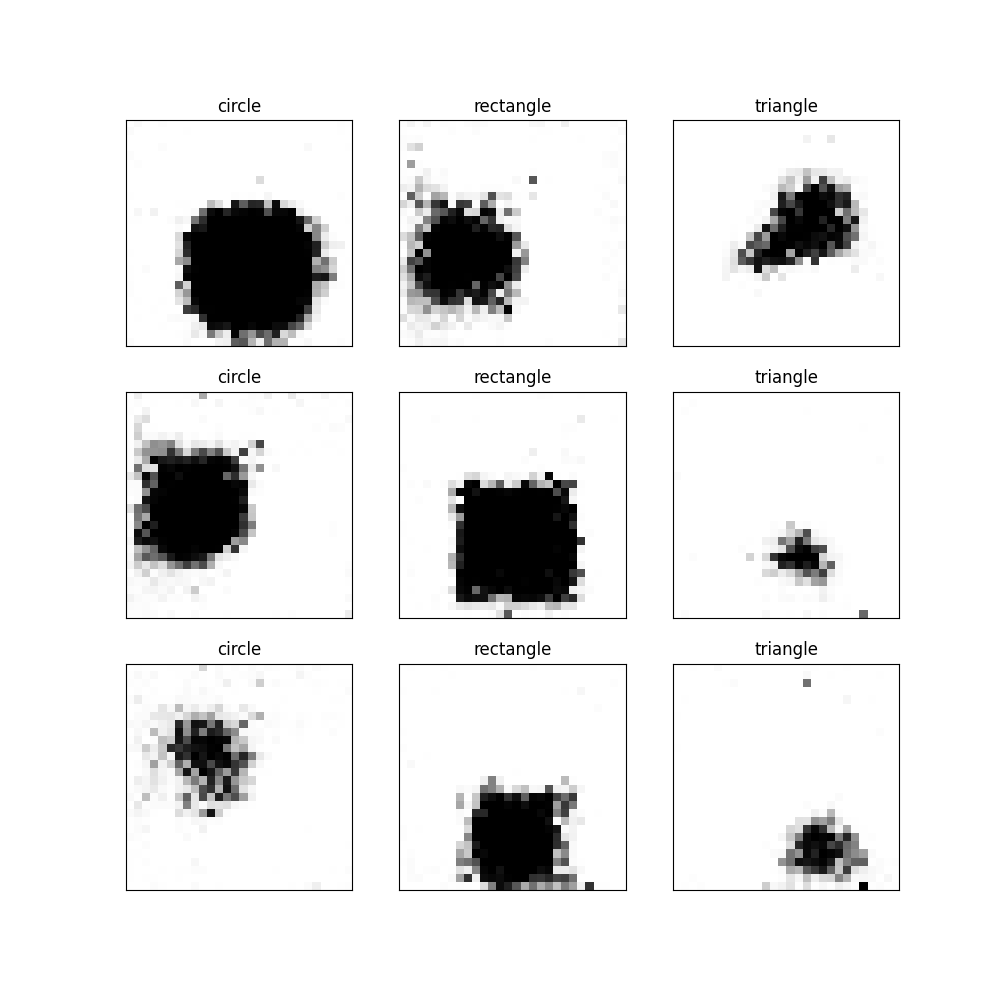
\includegraphics[width=0.45\linewidth]{kapitel/5_ergebnisse/densegan/good_example.png}}
	\qquad
	\subfloat[][]{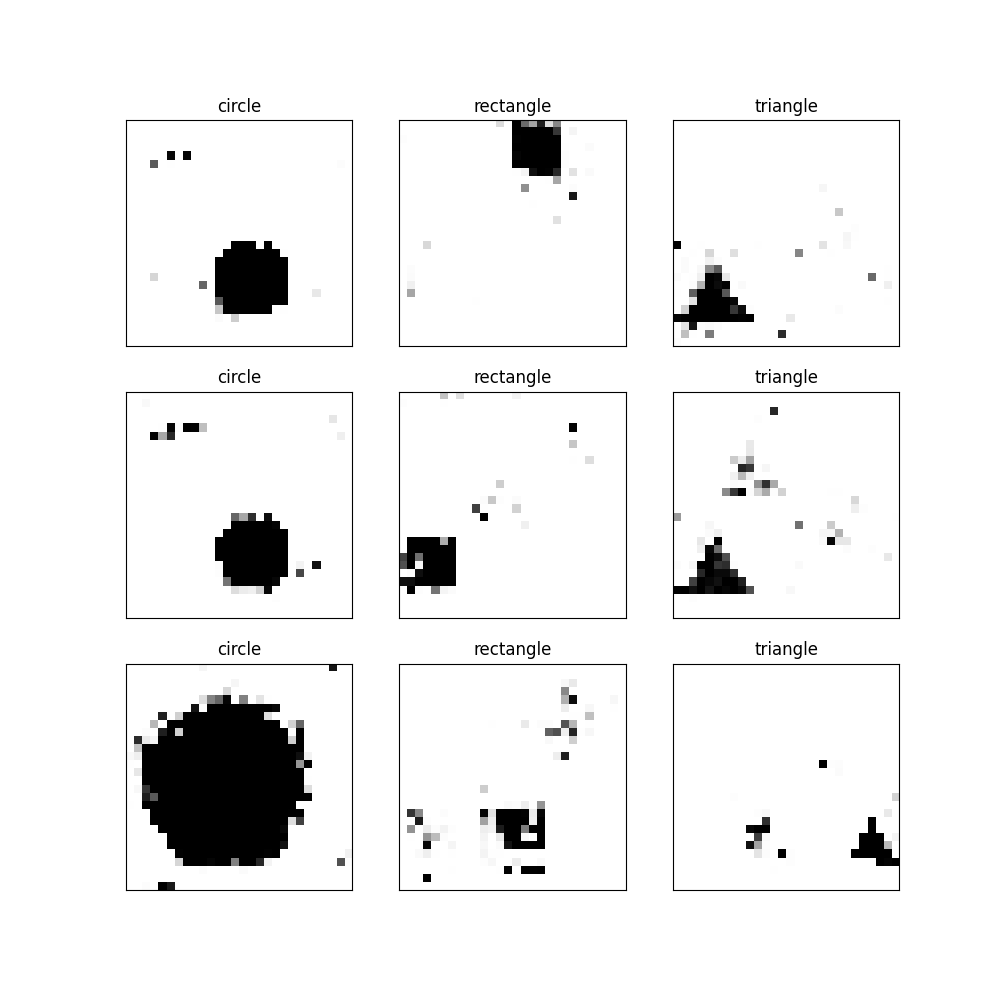
\includegraphics[height=0.35\textheight]{kapitel/5_ergebnisse/densegan/good_example_long.png}}
	\label{ergebnis:densegan-zusammenfassung}
	\caption[]{\textbf{a)} die subjektiv besten Ergebnisse nach regulärem Training; \textbf{b)} Ergebnisse nach zusätzlichem Training; \\auf beiden Bildern lässt sich starkes Rauschen erkennen}
\end{figure}

\subsubsection{DC GAN}
Probleme mit Rauschen existieren beim DC-GAN fast gar nicht, die Figuren sind alle sehr klar abgebildet.
Es existieren auch vergleichsweise wenig zusätzliche Pixelfragmente.
Die existierenden Pixelfragmente sind eher vergleichbar mit einer zweiten Figur auf dem Bild, da sie in Größe und Merkmalen nicht von der eigentlichen Figur zu unterscheiden sind.
Entsprechende Beispiele sind im \cref{ergebnis:dcgan-fid-zusammenfassung} zu sehen.
\newline

Allerdings ist die Qualität der DC-GAN-Bilder deutlich schlechter.
Oftmals wird eine Figur erzeugt, die Merkmale mehrere Kategorien besitzt.
Dabei handelt es sich zum Beispiel um einen Kreis mit einer geraden Kante oder Ecke.
Durch die Verschmelzung von Eigenschaften lassen sich die Figuren nicht immer eindeutig den geometrischen Formen zuordnen.

\begin{figure}[H]
	\centering
	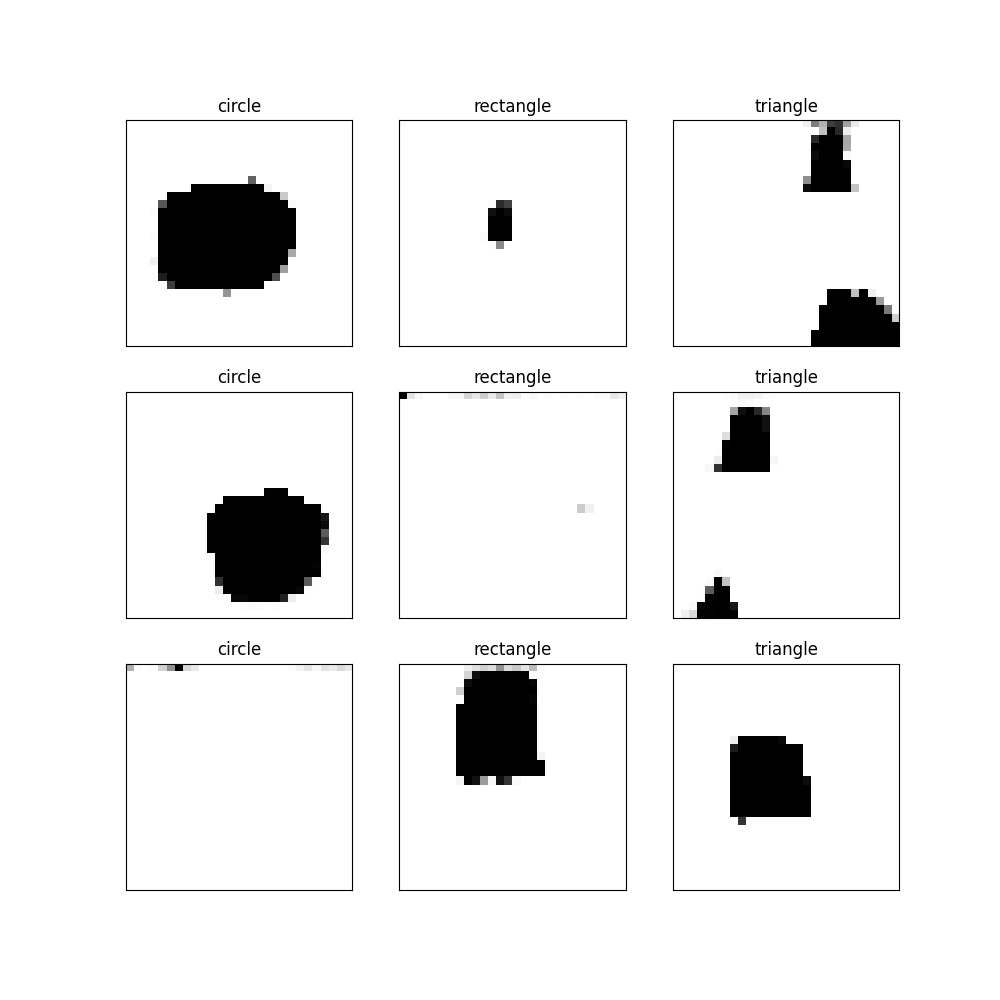
\includegraphics[width=0.45\linewidth]{kapitel/5_ergebnisse/dcgan/fid_circle.png}
	\label{ergebnis:dcgan-fid-zusammenfassung}
	\caption[]{\textbf{Oben Links:} ein Kreis mit einer geraden Kante; \textbf{Mitte Rechts:} zwei Pixelfragmente mit den schrägen Kanten eines Dreiecks}
\end{figure}

\subsubsection{Vergleich}
Insgesamt sind die Bilder des Dense GANs leicht besser als die Bilder des DC GANs.
Zwar sind sie deutlich verrauschter, aber die Figuren entsprechen mehr dem zugehörigen Label.
Beide Architekturen generieren jedoch keine Bilder, die von Menschen mit den Trainingsdaten verwechselt werden könnten.


\section{Interpretation der Ergebnisse}
Beide Architekturen erzeugen Bilder, die Gemeinsamkeiten mit den Trainingsdaten aufzeigen.
Unterschiede gibt es vor allem beim Rauschen und der Unterscheidbarkeit der Figuren.

\subsubsection{Rauschen}
Das Dense-GAN hat größere Probleme mit Rauschen.
Das lässt sich auf die Layerarchitektur zurück führen, da im Gegensatz zu Convolutional Layern die Pixel separater betrachtet werden.
Dadurch werden Zusammenhänge zwischen benachbarten Pixeln werden nicht so stark gefördert, wie beim DC GAN.
Allerdings werden beim DC GAN stattdessen vermehrt zusätzliche Figuren erzeugt.
Beim Dense GAN werden hingegen eher einzelne Pixel falsch eingefärbt.

\subsubsection{Unterscheidbarkeit der Formen}
Beide GANs neigen zur Vermischung von Eigenschaften unterschiedlicher Figuren, zum Beispiel ein Kreis mit einer geraden Kante.
Das könnte auch an der Ähnlichkeit der Kreise und Quadrate im kleinen Pixelformat liegen.
Die Schwierigkeiten beim Erzeugen von Dreiecken könnte auch damit zu tun haben, da sich die Figur stärker von den anderen beiden unterscheidet.
Durch das exemplarische Zusatztraining beim Dense GAN nehmen die Ähnlichkeiten zwischen den Figuren aber ab und die besonderen Besonderheiten der einzelnen Figuren werden stärker hervorgehoben.

\section{Beschränkung der Forschung}
Für das Training und somit auch die Ergebnisse war insbesondere die verfügbare Hardware ein große Beschränkung.
Mit besserer Hardware hätten unter anderem mehr Hyperparameterkombinationen ausprobiert oder ein deutlich längeres Training durchgeführt werden.
Weitere Trainingsdurchläufe haben sich prototypisch ausch schon beim Dense GAN bewährt und sind deshalb vielversprechend.
\newline

Die Trainingsdaten besitzen auch kein Bildrauschen oder ähnliche Verfälschungen.
Das würde das Training zusätzlich erschweren, aber gleichzeitig die entstehenden Netze robuster machen.
Dadurch können dann auch die Ergebnisse für unverfälschte Bilder verbessert werden.

\section{Fazit}
Es konnten 2 GAN Architekturen gefunden werden, die beide Ergebnisse erzeugen.
Die Verwendung eines Dense GANs hat sich im beschränkten Training mit 100 Epochen als besser erwiesen.
Abbildungen der verwendeten Architektur befinden sich im Anhang: \cref{architecture:densegan-dis} und \cref{architecture:densegan-gen}.
Ein intensiveres Training könnte aber nochmals bessere Ergebnisse hervorbringen.

\section{Ausblick}
Für zukünftige Forschung lassen sich insbesondere die Trainingsdaten weiter anpassen und die angesprochene Verfälschung der Bilder einbauen.
Außerdem besteht die Möglichkeit die Figuren auf den Figuren alle zu zentrieren und skalieren, sodass sie das Bild komplett ausfüllen.

Das ist insofern interessant, als dass das ohne Neuronale Netze und alleine durch Algorithmen möglich ist.
Es wird also kein extra Training benötigt und die Bilder können dementsprechend in der Vorverarbeitung angepasst werden.
So könnte ein Vergleich zwischen vorverarbeiteten und unvorverarbeiteten Daten gezogen werden.
\newline

Des Weiteren können die vorgestellten Architekturen weiter trainiert werden.
Wie durch das Dense GAN gezeigt, können die Ergebnisse mit mehr Training noch weiter verbessert werden.
Zusätzlich könnten bei viel Hardware Kapazitäten auch die Hyperparameter noch einmal mit dem Genetic Algorithm optimiert werden.
Dadurch könnten noch weitere eventuell überraschende Hyperparameterkombinationen gefunden werden.

	%!TEX root = ../../main.tex

\chapter{Zusammenfassung}
	
	\cleardoublepage{}
	\appendix
	\pagenumbering{Roman}
	\chapter{Anhang}
\newpage

\section{Dense GAN Architektur}
\begin{figure}[H]
	\centering
	\includegraphics[height=0.9\textheight]{kapitel/5\_ergebnisse/architectures/densegan\_discriminator.png}
	\caption{Dense GAN - Architektur Discriminator}
	\label{architecture:densegan-dis}
\end{figure}

\begin{figure}[H]
	\centering
	\includegraphics[height=\textheight]{kapitel/5\_ergebnisse/architectures/densegan\_generator.png}
	\caption{Dense GAN - Architektur Generator}
	\label{architecture:densegan-gen}
\end{figure}

\section{DCGAN Architektur}

\begin{figure}[H]
	\centering
	\includegraphics[height=0.9\textheight]{kapitel/5\_ergebnisse/architectures/dcgan\_discriminator.png}
	\caption{DC GAN - Architektur Discriminator}
	\label{architecture:dcgan-dis}
\end{figure}

\begin{figure}[H]
	\centering
	\includegraphics[height=\textheight]{kapitel/5\_ergebnisse/architectures/dcgan\_generator.png}
	\caption{DC GAN - Architektur Generator}
	\label{architecture:dcgan-gen}
\end{figure}


	% <---  content end  --->
	
	\printbibliography[heading=bibintoc]
\end{document}